\section{}

\textbf{Tiempo de lectura:} \{s17-reading-time\}

La \textbf{memoria virtual}{} es una técnica que permite la ejecución de
procesos sin que estos tengan que ser cargados completamente en la
memoria.

Los programas suelen tener partes de código que rara vez son ejecutadas.
Por ejemplo, las funciones para manejar condiciones de error que, aunque
útiles, generalmente nunca son invocadas. También es frecuente que se
reserve más memoria para datos de lo que realmente es necesario. Por
ejemplo, muchos programadores tienen la costumbre de hacer cosas tales
como declarar un \emph{array} de 65536 elementos, cuando realmente solo
necesitan 255. Teniendo todo esto en cuenta, y con el fin de mejorar el
aprovechamiento de la memoria, parece que sería interesante no tener que
cargar todas las porciones de los procesos y que, aún así, pudieran
ejecutarse. Eso es exactamente lo que proporciona la \textbf{memoria
virtual}.

La habilidad de ejecutar un proceso cargado parcialmente en memoria
proporciona algunos beneficios importantes:

\begin{itemize}
\item
  Un programa nunca más estaría limitado por la cantidad de memoria
  disponible.

  Es decir, los desarrolladores pueden escribir programas considerando
  que disponen de un espacio de direcciones virtual extremadamente
  grande, sin considerar la cantidad de memoria realmente disponible. No
  debemos olvidar que sin memoria virtual, para que un proceso pueda ser
  ejecutado, debe estar completamente cargado en la memoria.
\item
  Puesto que cada programa ocupa menos memoria, más programas se pueden
  ejecutar al mismo tiempo; con el correspondiente incremento en el uso
  de la CPU y en el rendimiento del sistema, pero sin efectos negativos
  en el tiempo de respuesta y en el de ejecución.
\end{itemize}

El concepto de \textbf{memoria virtual} no debe confundirse con el de
\textbf{espacio de direcciones virtual}. Sin embargo están relacionados,
puesto que el que exista separación entre la memoria física y la manera
en la que los procesos perciben la memoria es un requisito para poder
implementar la memoria virtual.

\section{Paginación bajo demanda}\label{_paginaciuxf3n_bajo_demanda}

La \textbf{paginación bajo demanda}{} es la técnica con la que
frecuentemente se implementa la \textbf{memoria virtual} en los sistemas
con paginación.

En la \textbf{paginación bajo demanda} las páginas individuales, en las
que se dividen los espacios de direcciones virtuales de los diferentes
procesos, pueden ser sacadas de la memoria de manera temporal y copiadas
a un almacenamiento de respaldo, para posteriormente volver a ser
traídas a la memoria cuando son necesitadas por su proceso. A este
proceso de guardado y recuperación de las páginas sobre el
almacenamiento de respaldo se lo denomina \textbf{{}intercambio} o
\textbf{\emph{{}swapping}} y es llevado a cabo por un componente del
sistema operativo denominado el \textbf{{}paginador}.

Para que se puedan cargar las páginas cuando son necesitadas por su
proceso, hace falta que el \textbf{paginador} sepa cuándo lo son. Eso
requiere que el hardware proporcione algún tipo de soporte, por ejemplo,
incorporando un \textbf{bit de válido}{} a la entrada de cada página en
la tabla de páginas, que se utiliza de la siguiente manera:

\begin{itemize}
\item
  Cuando el \textbf{bit de válido} está a 1 la página es legal y está en
  la memoria. Es decir, la página existe en el espacio de direcciones
  virtual del proceso y tiene asignado un marco de memoria física.
\item
  Cuando el \textbf{bit de válido} está a 0, pueden ocurrir varias
  cosas:

  \begin{itemize}
  \item
    La página es legal, pero está almacenada en disco y no en la
    memoria.
  \item
    La página no es legal. Es decir, no existe en el espacio de
    direcciones virtual del proceso.

    Esto puede ser debido a que la página esté en un hueco del espacio
    de direcciones ---en una región que no está siendo utilizada--- por
    lo que el sistema operativo no le ha asignado espacio de
    almacenamiento ni en disco ni en la memoria.
  \end{itemize}
\end{itemize}

Si un proceso accede a una página legal, no ocurre nada y la instrucción
se ejecuta con normalidad. Pero si accede a una página marcada como
inválida:

\begin{enumerate}
\def\labelenumi{\arabic{enumi}.}
\item
  Al intentar acceder a la página, la MMU comprueba el bit de válido y
  genera una excepción de \textbf{{}fallo de página} al estar marcada
  como inválida. Dicha excepción es capturada por el sistema operativo.
\item
  El sistema operativo comprueba en una tabla interna si la página es
  legal o no. Es decir, si la página realmente no pertenece al espacio
  de direcciones virtual del proceso o si pertenece, pero está
  almacenada en el disco. Esta tabla interna suele almacenarse en el PCB
  del proceso como parte de la información de gestión de la memoria.
\item
  Si la página es ilegal, el proceso ha cometido un error y debe ser
  terminado. En sistemas POSIX, por ejemplo, el sistema envía al proceso
  una señal de \textbf{violación de segmento} que lo obliga a terminar.
\item
  Si la página es legal, se carga desde el disco:

  \begin{enumerate}
  \def\labelenumii{\alph{enumii}.}
  \item
    El núcleo busca un marco de memoria libre que, por ejemplo, se puede
    escoger de la lista de marcos libres del sistema.
  \item
    Se solicita una operación de disco para leer la página deseada en el
    marco asignado.

    Puesto que no resulta eficiente mantener la CPU ocupada mientras la
    página es recuperada desde el disco, el sistema debe solicitar la
    lectura de la página y poner al proceso en estado
    \textbf{esperando}.
  \item
    Cuando la lectura del disco haya terminado, se modifica la tabla
    interna, antes mencionada, y la tabla de páginas para indicar que la
    página está en la memoria.
  \item
    Reiniciar la instrucción que fue interrumpida por la excepción.
    Generalmente esto se hace colocando el proceso nuevamente en la
    \textbf{cola de preparados} y dejando que el \textbf{asignador} lo
    reinicie cuando sea escogido por el \textbf{planificador} de la CPU.
  \end{enumerate}
\end{enumerate}

Un caso extremo de la paginación bajo demanda es la \textbf{paginación
bajo demanda pura}{}. En ella la ejecución de un proceso se inicia sin
cargar ninguna página en la memoria. Cuando el sistema operativo sitúa
el contador de programa en la primera instrucción del proceso ---que es
una página no residente en memoria--- se genera inmediatamente un
\textbf{fallo de página}. La página es cargada en la memoria ---tal y
como hemos descrito anteriormente--- y el proceso continúa ejecutándose,
fallando cuando sea necesario con cada página que necesite y no esté
cargada. Las principales ventajas de la \textbf{paginación bajo demanda
pura} son:

\begin{itemize}
\item
  Nunca se trae desde el disco una página que no sea necesaria.
\item
  El inicio de la ejecución de un proceso es mucho más rápido que si se
  cargara todo el proceso desde el principio.
\end{itemize}

\subsection{Requerimientos de la paginación bajo
demanda}\label{_requerimientos_de_la_paginaciuxf3n_bajo_demanda}

Los requerimientos hardware para que un sistema operativo pueda soportar
la \textbf{paginación bajo demanda} son:

\begin{itemize}
\item
  Tabla de páginas con habilidad para marcar entradas inválidas, ya sea
  utilizando un bit específico o con valores especiales en los bits de
  protección.
\item
  Disponibilidad de un dispositivo de almacenamiento secundario.

  En este dispositivo se guardan las páginas que no están presentes en
  la memoria principal. Normalmente se trata de un disco conocido como
  \textbf{{}dispositivo de intercambio}, mientras que la sección de
  disco utilizada concretamente para dicho propósito se conoce como
  \textbf{espacio de intercambio}{} o \textbf{\emph{swap}}.
\item
  Posibilidad de reiniciar cualquier instrucción después de un fallo de
  página.

  En la mayor parte de los casos esta funcionalidad es sencilla de
  conseguir. Sin embargo, la mayor dificultad proviene de las
  instrucciones que pueden modificar diferentes posiciones de la
  memoria, como aquellas pensadas para mover bloques de bytes o
  palabras. En el caso de que el bloque de origen o de destino atraviese
  un borde de página, la instrucción sería interrumpida cuando la
  operación solo haya sido realizada parcialmente. Si además ambos
  bloques se superpusieran, no se podría reiniciar la instrucción
  completa. Las posibles soluciones a este problema deben ser
  implementadas en la CPU.
\end{itemize}

\subsection{Rendimiento de la paginación bajo
demanda}\label{_rendimiento_de_la_paginaciuxf3n_bajo_demanda}

Indudablemente, el rendimiento de un sistema con \textbf{paginación bajo
demanda} se ve afectado por el \textbf{número de fallos de páginas}. En
el peor de los casos, en cada instrucción un proceso puede intentar
acceder a una página distinta, empeorando notablemente el rendimiento.
Sin embargo, esto no ocurre, puesto que los programas tienden a tener
localidad de referencia (véase el
\hyperref[_hiperpaginaciuxf3n]{Hiperpaginación}).

\subsubsection{Tiempos de acceso
efectivo}\label{_tiempos_de_acceso_efectivo}

Como con la \textbf{paginación}, el rendimiento de un sistema con
\textbf{paginación bajo demanda} también está relacionado con el
concepto de \textbf{tiempo de acceso efectivo}{} a la memoria, que
intenta estimar el tiempo que realmente se tarda en acceder a la memoria
teniendo en cuenta mecanismos del sistema operativo.

Supongamos que conocemos el tiempo de acceso a la memoria cuando hay
acierto de página -\/-es decir, si no ocurre un fallo de página-\/- al
que llamaremos \(T_text(eap)\), y que conocemos la probabilidad
\(p_text(fp)\) de que ocurra un fallo de página. Entonces, el
\textbf{tiempo de acceso efectivo} se podría calcular como la
probabilidad de que no ocurra un fallo de página \((1 - p_text(fp))\)
por el \textbf{tiempo de acceso} a la memoria en dicho caso
\(T_text(eap)\), más la probabilidad de que ocurra un fallo de página
\(p_text(fp))\) por el tiempo necesario para gestionar cada fallo de
página ---o \textbf{tiempo de fallo de página}{}--- \(T_text(fp)\):

\[T_"em" = (1-p_"fp")*T_"eap" + p_"fp"*T_"fp"\]

Por tanto, para calcular el \textbf{tiempo de acceso efectivo}
\(T_text(em)\) necesitamos estimar el \textbf{tiempo de fallo de página}
\(T_text(fp)\), que se consume fundamentalmente en:

\begin{itemize}
\item
  Servir la excepción de fallo de página.

  Esto incluye capturar la interrupción, salvar los registros y el
  estado del proceso, determinar que la interrupción es debida a una
  excepción de \textbf{fallo de página}, comprobar si la página es legal
  y determinar la localización de la misma en el disco. Aproximadamente,
  en realizar esta tarea el sistema puede tardar de 1 a 100 μs.
\item
  Leer la página en un marco libre. En esta tarea se puede tardar
  alrededor de 8 ms, pero este tiempo puede ser mucho mayor si el
  dispositivo está ocupado y se debe esperar a que se realicen otras
  operaciones.
\item
  Reiniciar el proceso. Si incluimos el tiempo de espera en la cola de
  preparados, se puede tardar entre 1 y 100 μs.
\end{itemize}

Como se puede apreciar, la mayor parte del \textbf{tiempo de fallo de
página} es debido al tiempo requerido para acceder al
\textbf{dispositivo de intercambio}.

Para ilustrar el cálculo del \textbf{tiempo de acceso efectivo} a la
memoria, solo vamos a considerar el tiempo requerido para acceder al
\textbf{dispositivo de intercambio}, ignorando las otras tareas a
realizar durante el \textbf{fallo de página}, ya que comparativamente
consumen mucho menos tiempo. Vamos a suponer que el \textbf{tiempo de
acceso} a la memoria en caso de acierto de página \(T_text(eap)\) es de
200 ns y que la probabilidad \(p_text(fp)\) es muy pequeña ---es decir,
\(p_text(fp) ll\)1---:

\[{:(T_"em", =, (1-p_"fp")*,200 "ns", +, p_"fp"*8 "ms" \qquad\qquad),
   (     , =, (1-p_"fp")*,200 "ns", +, p_"fp"*8000000 "ms"),
   (     , ~~,          ,200 "ns", +, 7999800 "ms"*p_"fp"),
   (     , ~~,          ,        ,  , 7999800 "ms"*p_"fp"):}\]

Como se puede apreciar el \textbf{tiempo de acceso efectivo}
prácticamente es proporcional a la \textbf{tasa de fallos de página}{}
\(tau_text(fp)\):

\[T_"em" ~~ T_"eap" + tau_"fp"\]

donde:

\[tau_text(fp)=p_text(fp) T_text(fp)\]

Por ejemplo, si un proceso causa un fallo de página en uno de cada 1000
accesos ---es decir, \(p_text(fp)= 0.001\) --- el \textbf{tiempo de
acceso efectivo} es de 8.2 ms, por lo que el rendimiento del sistema es
40 veces inferior debido a la \textbf{paginación bajo demanda}. Por
tanto, es necesario mantener la \textbf{tasa de fallos de página}
\(tau_text(fp)\) lo más baja posible para mantener un rendimiento
adecuado.

Respecto a \(T_text(eap)\), el \textbf{tiempo de acceso} a la memoria en
caso de acierto de página no se corresponde directamente con el tiempo
de acceso a la memoria física \(T_text(m)\), porque estamos en un
sistema que utiliza paginación -\/-que recordemos que necesita varios
accesos para cada dirección de memoria virtual-\/- y que puede usar una
TLB para mejorar su rendimiento. Por tanto, \(T_text(eap))\) es el
\textbf{tiempo de acceso efectivo} \(T_text(em))\) que calculamos en el
\hyperref[paginaciuxf3n]{???}.

Por ejemplo, en el \hyperref[_tiempos_de_acceso_a_la_memoria]{???} vimos
que el \textbf{tiempo de acceso efectivo} para el \textbf{método básico
de paginación} con \textbf{TLB} era:

\[T_"em" = (2-p_"TLB")*T_"m" + T_"TLB"\]

donde \(p_text(TLB)\) es la probabilidad de que una entrada esté en la
\textbf{TLB} y \(T_text(m)\) es el \textbf{tiempo de acceso} a la
memoria física. Si sustituimos esta expresión por el \(T_text(eap)\) en:

\[{:(T_"em", ~~, T_"eap" \qquad\qquad\qquad\qquad\ ,+ tau_"fp"),
  (      , ~~, (2-p_"TLB")*T_"m" + T_"TLB" ,+ tau_"fp"):}\]

que nos daría el \textbf{tiempo de acceso efectivo} a la memoria en
\textbf{paginación bajo demanda} con una \textbf{tabla de páginas
lineal} y \textbf{TLB}.

Mientras que si sustituimos el \textbf{tiempo de acceso efectivo}
calculado en el \hyperref[_tiempos_de_acceso_a_la_memoria_2]{???}:

\[T_"em" = ((1-p_"TLB")*n+1)*T_"m" + T_"TLB"\]

obtenemos el \textbf{tiempo de acceso efectivo} a la memoria en
\textbf{paginación bajo demanda} con \textbf{paginación jerárquica} de
\emph{n} niveles:

\[T_"em" ~~ ((1-p_"TLB")*n+1)*T_"m" + T_"TLB" + tau_"fp"\]

Sin embargo, debemos recordar que para obtener ambas expresiones estamos
simplificando bajo la suposición de que \(p_text(fp) ll\) 1. Si no
podemos hacer esta suposición, podemos volver a la expresión original
para \(T_text(em)\), antes de la simplificación:

\[T_"em" = (1-p_"fp")*T_"eap" + p_"fp"*T_"fp"\]

y repetir la sustitución de \(T_text(eap)\) por las expresiones para
\(T_text(em)\) calculadas en el
\hyperref[_tiempos_de_acceso_a_la_memoria]{???} y el
\hyperref[_tiempos_de_acceso_a_la_memoria_2]{???}. Así obtenemos que el
\textbf{tiempo de acceso efectivo} \(T_text(em)\) para \textbf{tabla de
páginas lineal} con \textbf{TLB} y \textbf{paginación bajo demanda} es:

\[{:(T_"em", =, (1-p_"fp")*T_"eap" \qquad\qquad\qquad\qquad\ \ \ , +, p_"fp"*T_"fp"),
    (    , =, (1-p_"fp")*[(2-p_"TLB")*T_"m" + T_"TLB"], +, tau_"fp"\qquad):}\]

Mientras que para la \textbf{paginación jerárquica} de \emph{n} niveles
es:

\[T_"em" = (1-p_"fp")*[((1-p_"TLB")*n+1)*T_"m" + T_"TLB"] + tau_"fp"\]

\subsubsection{Manejo y uso del espacio de
intercambio}\label{_manejo_y_uso_del_espacio_de_intercambio}

Otro aspecto fundamental que afecta al rendimiento de la
\textbf{paginación bajo demanda} es el uso del espacio de intercambio.

Cuando un proceso genera un \textbf{fallo de página}, el sistema
operativo debe recuperar la página de allí donde esté almacenada. Si
esto ocurre al principio de la ejecución, ese lugar seguramente será el
archivo que contiene la imagen binaria del programa, pues es donde se
encuentran las páginas en su estado inicial. Sin embargo, el acceso al
espacio de intercambio es mucho más eficiente que el acceso a un sistema
de archivos, incluso aunque el primero esté almacenado dentro de un
archivo de gran tamaño. Esto es debido a que los datos se organizan en
bloques contiguos de gran tamaño, se evitan las búsquedas de archivos y
las indirecciones en la asignación de espacio. Por ello debemos
plantearnos qué hacer con las imágenes de los programas que van a ser
ejecutados.

\begin{itemize}
\item
  Se puede mejorar el rendimiento copiando en el espacio de intercambio
  la imagen completa de los programas durante el inicio del proceso,
  para después realizar la \textbf{paginación bajo demanda} sobre dicha
  copia.
\item
  Otra alternativa es cargar las páginas desde el archivo que contiene
  la imagen cuando son usadas por primera vez, pero siendo escritas en
  el espacio de intercambio cuando dichas páginas tienen que ser
  reemplazadas. Esta aproximación garantiza que solo las páginas
  necesarias son leídas desde el sistema de archivos, reduciendo el uso
  de espacio de intercambio, mientras que las siguientes operaciones de
  intercambio se hacen sobre dicho espacio.
\item
  También se puede suponer que el código de los procesos no puede
  cambiar. Esto permite utilizar el archivo de la imagen binaria para
  recargar las páginas de código, lo que también evita escribirlas
  cuando son sustituidas. Sin embargo, el espacio de intercambio se
  sigue utilizando para las páginas que no están directamente asociadas
  a un archivo, como la pila o el montón de los procesos.

  Este último método parece conseguir un buen compromiso entre el tamaño
  del espacio de intercambio y el rendimiento. Por eso se utiliza en la
  mayor parte de los sistemas operativos modernos.
\end{itemize}

\section{Copy-on-write}\label{_copy_on_write}

{} El \textbf{\emph{copy-on-write}} o \textbf{copia durante la
escritura} permite la creación rápida de nuevos procesos, minimizando la
cantidad de páginas que deben ser asignadas a estos.

Para entenderlo, es importante recordar que la llamada al sistema
\{linux\_fork\} crea un proceso hijo cuyo espacio de direcciones es un
duplicado del espacio de direcciones del padre. Indudablemente, esto
significa que durante la llamada es necesario asignar suficientes marcos
de memoria física como para alojar las páginas del nuevo proceso hijo.
El \textbf{\emph{copy-on-write}} minimiza de la siguiente manera el
número de marcos que deben ser asignadas al nuevo proceso:

\begin{figure}
\centering
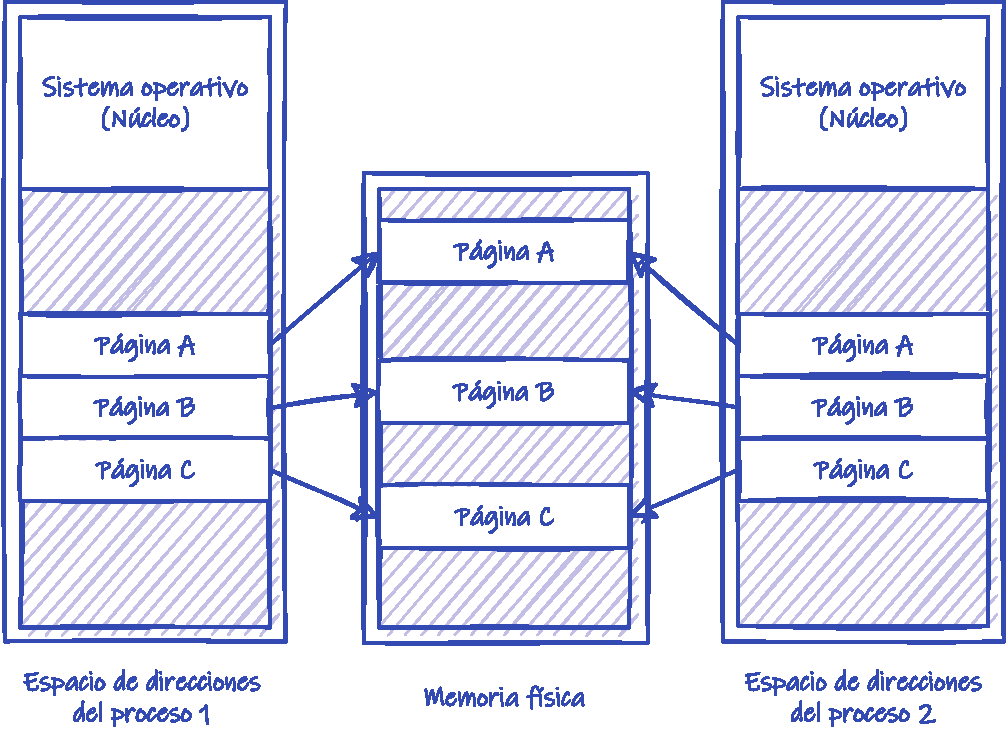
\includegraphics[width=0.8\textwidth]{media/C17_memoria_virtual/copy_on_write1.pdf}
\caption{Copy-on-write antes de que el proceso 1 modifique la página
A.}\label{fig-copy-on-write-1}
\end{figure}

\begin{enumerate}
\def\labelenumi{\arabic{enumi}.}
\item
  Cuando la llamada al sistema \{linux\_fork\} crea el nuevo proceso lo
  hace de forma que este comparta todas sus páginas con las del padre
  (véase la \hyperref[fig-copy-on-write-1]{Copy-on-write antes de que el
  proceso 1 modifique la página A.}).

  Sin el \textbf{\emph{copy-on-write}} el \{linux\_fork\} tendría que
  asignar marcos de memoria física al hijo, para a continuación copiar
  las páginas del padre en ellos. Sin embargo, con el
  \textbf{\emph{copy-on-write}} padre e hijo mapean sus páginas en los
  mismos marcos, evitando tener que asignar memoria libre.
\item
  Las páginas compartidas se marcan como \textbf{\emph{copy-on-write}}.

  Para ello se pueden marcar todas las páginas como de \textbf{solo
  lectura} en la tabla de páginas de ambos procesos y utilizar una tabla
  interna alojada en el PCB para indicar cuáles son realmente de solo
  lectura y cuáles están en \textbf{\emph{copy-on-write}}. Es importante
  destacar que realmente solo las páginas que pueden ser modificadas se
  marcan como \textbf{\emph{copy-on-write}}. Las páginas que no pueden
  ser modificadas ---por ejemplo, las que contienen el código ejecutable
  del programa--- simplemente pueden ser compartidas como de solo
  lectura por los procesos, como hemos comentado anteriormente.
\item
  Si algún proceso intenta escribir en una página
  \textbf{\emph{copy-on-write}}, la MMU genera una excepción para
  notificar el suceso al sistema operativo. Siguiendo lo indicado en el
  punto anterior, la excepción se originaría porque la página está
  marcada como de solo lectura, por lo que el sistema operativo
  comprobará si se trata de un acceso a una página
  \textbf{\emph{copy-on-write}} o a un intento real de escribir en una
  página de solo lectura. Para ello, el sistema solo tiene que mirar la
  tabla interna almacenada en el PCB. Si se ha intentado escribir en una
  página de solo lectura, el proceso ha cometido un error y generalmente
  será terminado.
\end{enumerate}

\begin{figure}
\centering
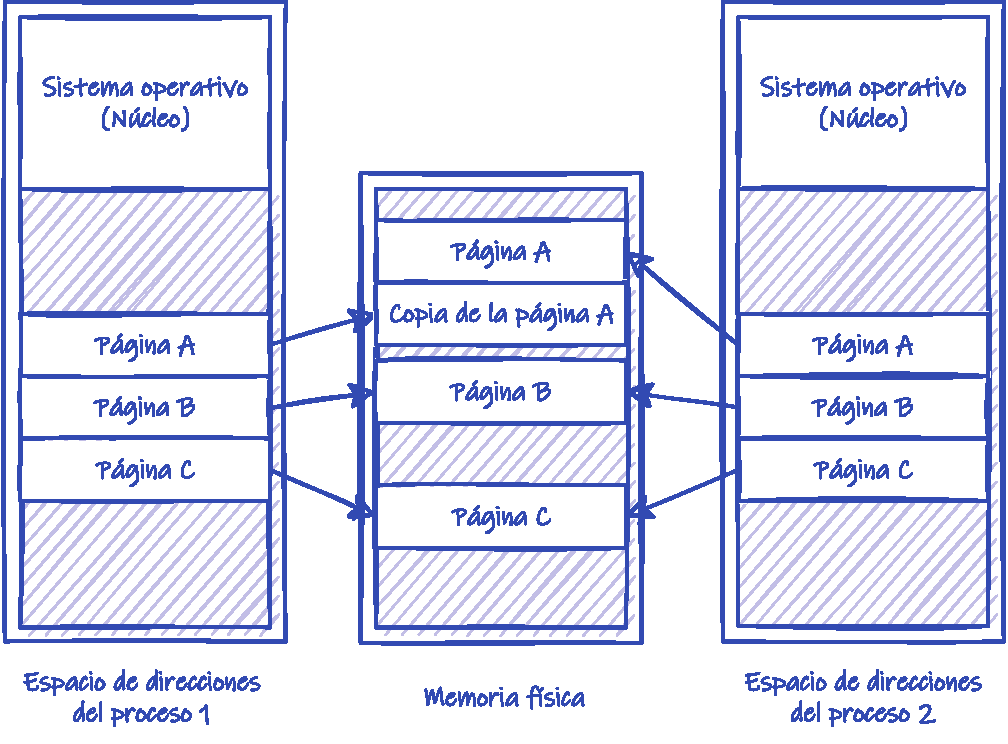
\includegraphics[width=0.8\textwidth]{media/C17_memoria_virtual/copy_on_write2.pdf}
\caption{Copy-on-write después de que el proceso 1 modifique la página
A.}\label{fig-copy-on-write-2}
\end{figure}

\begin{enumerate}
\def\labelenumi{\arabic{enumi}.}
\item
  Si el sistema detecta una escritura a una página de
  \textbf{\emph{copy-on-write}} solo tiene que copiarla en un marco
  libre y mapearlo en el espacio de direcciones del proceso (véase la
  \hyperref[fig-copy-on-write-2]{Copy-on-write después de que el proceso
  1 modifique la página A.}).

  Para esto se sustituye la página compartida por otra que contiene una
  copia, pero que ya no está compartida. Obviamente, la nueva página
  debe ser marcada como de escritura para que en el futuro pueda ser
  modificada por el proceso.
\item
  La página original marcada como \textbf{\emph{copy-on-write}} puede
  ser marcada como de escritura y no como \textbf{\emph{copy-on-write}},
  pero solo si no va a seguir siendo compartida. Esto es así porque una
  página marcada como \textbf{\emph{copy-on-write}} puede estar siendo
  compartida con otros procesos.
\item
  El sistema operativo puede reiniciar el proceso. A partir de ahora,
  este puede escribir en la página sin afectar al resto de los procesos.
  Sin embargo, puede seguir compartiendo otras páginas en
  \textbf{\emph{copy-on-write}}.
\end{enumerate}

El \textbf{\emph{copy-on-write}} permite ahorrar memoria y tiempo en la
creación de los procesos, puesto que solo se copian las páginas que son
modificadas por estos. Por eso se trata de una técnica común en
múltiples sistemas operativos, como por ejemplo los sistemas POSIX
modernos y Microsoft Windows.

El \textbf{\emph{copy-on-write}} es especialmente interesante si a
continuación se va a utilizar la llamada al sistema \{linux\_exec\}
puesto que si es así, copiar el espacio de direcciones completo es una
pérdida de tiempo.

El \textbf{\emph{copy-on-write}} también permite a los sistemas modernos
ahorrar memoria durante la reserva de grandes cantidades de memoria.
Cuando un proceso pide reservar páginas de memoria, generalmente los
sistemas deben proporcionar páginas con marcos sobreescritos con ceros,
para evitar exponer los datos del proceso que los utilizó anteriormente.
En previsión de esto, el sistema mantiene un marco completamente a 0 y
durante las reservas de memoria proporciona páginas en
\textbf{\emph{copy-on-write}} sobre dicho marco a 0. De esta forma, se
ahorra memoria física y tiempo de CPU, puesto que realmente no se asigna
un marco de memoria física y se pone a 0 su contenido hasta el momento
en el que el proceso intenta escribir en una página de memoria
previamente reservada.

\section{Archivos mapeados en
memoria}\label{_archivos_mapeados_en_memoria}

{} Los \textbf{archivos mapeados en memoria} permiten acceder a un
archivo como parte del espacio de direcciones virtuales de un proceso.
Algunas de las características de esta técnica son:

\begin{itemize}
\item
  Cuando una región del espacio de direcciones queda marcada para ser
  mapeada sobre una región de un archivo, se utiliza una estrategia
  similar a la comentada para el método básico de la paginación bajo
  demanda. La diferencia es que las páginas son cargadas desde dicho
  archivo y no desde el espacio de intercambio. Es decir, en un primer
  acceso a una página mapeada se produce un \textbf{fallo de página} que
  es resuelto por el sistema operativo leyendo una porción del archivo
  en el marco asignado a la página.
\item
  Esto significa que la lectura y escritura del archivo se realiza a
  través de lecturas y escrituras en la memoria, lo que simplifica el
  acceso y elimina el costo adicional de las llamadas al sistema:
  \{linux\_read\}, \{linux\_write\}, etc.
\item
  Las escrituras en disco se suelen realizar de forma asíncrona. Es
  decir, los datos no se escriben inmediatamente en disco cuando se
  modifica la página, sino que el sistema operativo comprueba
  periódicamente las páginas modificadas y las escribe en disco.
\item
  Los marcos utilizados en el mapeo pueden ser compartidos, lo que
  permite compartir los datos de los archivos. Además, se puede incluir
  soporte de \textbf{\emph{copy-on-write}}, lo que permite a los
  procesos compartir buena parte de un archivo en modo de solo lectura,
  pero disponiendo de sus propias copias de aquellas páginas que
  modifiquen.

  Indudablemente, para que los procesos puedan compartir datos es
  necesario que exista algún tipo de coordinación (véase el
  \hyperref[sincronizaciuxf3n]{???}).
\end{itemize}

\subsection{Ejemplo de mapeo de
archivos}\label{_ejemplo_de_mapeo_de_archivos}

Tanto en los sistemas POSIX como en Windows API el archivo a mapear hay
que abrirlo con la llamada al sistema destinada a ello. Por ejemplo, en
sistemas POSIX:

\begin{Shaded}
\begin{Highlighting}[]
\DataTypeTok{int}\NormalTok{ fd }\OperatorTok{=}\NormalTok{ open}\OperatorTok{(} \StringTok{"foo.txt"}\OperatorTok{,}\NormalTok{ O\_RDONLY }\OperatorTok{);}
\end{Highlighting}
\end{Shaded}

En la API POSIX con esto es suficiente para usar la llamada al sistema
\{linux\_mmap\} y mapear el archivo en memoria:

\begin{Shaded}
\begin{Highlighting}[]
\DataTypeTok{int}\NormalTok{ length }\OperatorTok{=}\NormalTok{ lseek}\OperatorTok{(}\NormalTok{ fd}\OperatorTok{,} \DecValTok{0}\OperatorTok{,}\NormalTok{ SEEK\_END }\OperatorTok{);}
\DataTypeTok{void}\OperatorTok{*}\NormalTok{ p }\OperatorTok{=}\NormalTok{ mmap}\OperatorTok{(}
\NormalTok{    NULL}\OperatorTok{,}
\NormalTok{    length}\OperatorTok{,}
\NormalTok{    PROT\_READ}\OperatorTok{,}
\NormalTok{    MAP\_SHARED}\OperatorTok{,}
\NormalTok{    fd}\OperatorTok{,}
    \DecValTok{0}
\OperatorTok{);}
\end{Highlighting}
\end{Shaded}

\begin{itemize}
\item
  Descriptor del archivo abierto con \{linux\_open\}.
\item
  La longitud de la región del archivo a mapear. Si queremos mapear todo
  el archivo, podemos usar \{linux\_lseek\} para conocer su longitud.
\item
  Si no se mapea todo el archivo, se puede indicar la posición del
  archivo donde comenzar el mapeo. Esta posición debe ser múltiplo del
  tamaño de página.
\item
  Permisos de la memoria mapeada. Deben coincidir con el modo con el que
  se abrió el archivo.
\end{itemize}

Una vez mapeado el archivo, si no se van a crear más mapeos, se puede
cerrar el descriptor de archivo con \{linux\_close\}. Y la región de
memoria mapeada se puede liberar, al terminar, con \{linux\_munmap\}.

En \{mapped\_files\_cpp\} se puede ver un ejemplo de un programa que
cuenta el número de líneas, palabra y caracteres de un archivo. Para
acceder al archivo, primero lo mapea en memoria, para así poder acceder
a su contenido sin tener que leerlo usando \{linux\_read\}. Una vez ha
terminado, libera la memoria mapeada.

Con Windows API el proceso requiere un paso más. Primero hay que usar el
manejador del archivo abierto para crear un \textbf{objeto de mapeo de
archivo} con \{win32\_createfilemapping\}. Después, el manejador
devuelto por \{win32\_createfilemapping\} es usado con
\{win32\_mapviewoffile\} para mapear el archivo en la memoria del
proceso.

Para liberar la memoria mapeada, se utiliza \{win32\_unmapviewoffile\}.
Mientras que para cerrar el manejador del \textbf{objeto de mapeo de
archivo} se usa \{win32\_closehandle\}, como es habitual.

\subsection{Mapeo de archivos en el
núcleo}\label{_mapeo_de_archivos_en_el_nuxfacleo}

Algunos sistemas operativos ofrecen el servicio de mapeo de archivos en
la memoria solo a través de una llamada al sistema concreta, permitiendo
utilizar las llamadas estándar ---\{linux\_read\}, \{linux\_write\},
etc.--- para hacer uso de la E/S tradicional. Sin embargo, muchos
sistemas modernos utilizan el mapeo en la memoria independientemente de
que se pidan o no.

Por ejemplo, en los sistemas POSIX, si un proceso utiliza llamada al
sistema \{linux\_mmap\} es porque explícitamente pide que el archivo sea
mapeado en memoria. Por tanto, el núcleo mapea el archivo en el espacio
de direcciones del proceso.

Pero en Linux, Microsoft Windows y otros sistemas operativos modernos,
adicionalmente, cuando un archivo es abierto con la llamada al sistema
estándar ---como \textbf{open}--- el archivo es mapeado en el espacio de
direcciones del núcleo y las llamadas \textbf{read} y \textbf{write} son
traducidas en accesos a la memoria en dicha región. No importa como sea
abierto el archivo. Estos sistemas tratan toda la E/S a archivos como
mapeada en memoria, permitiendo que el acceso a los mismos, tenga lugar
a través del eficiente componente de gestión de la memoria.

\section{Reemplazo de página}\label{_reemplazo_de_puxe1gina}

Hasta el momento hemos considerado que disponemos de memoria física
suficiente para atender cualquier fallo de página, pero ¿qué ocurre
cuando no quedan marcos libres?. En ese caso el código que da servicio a
la excepción de \textbf{fallo de página} debe escoger alguna página,
intercambiarla con el disco y utilizar el marco de la misma para cargar
la nueva página. Es decir, debemos modificar la función que ejecuta los
pasos descritos en el \hyperref[_paginaciuxf3n_bajo_demanda]{Paginación
bajo demanda} de la siguiente manera:

\begin{enumerate}
\def\labelenumi{\arabic{enumi}.}
\item
  Si la página es legal, debe ser cargada desde el disco.

  \begin{enumerate}
  \def\labelenumii{\alph{enumii}.}
  \item
    Buscar la localización de la página en disco.
  \item
    El núcleo debe buscar un marco de memoria libre que, por ejemplo, se
    puede escoger de la lista de marcos libres del sistema.

    \begin{enumerate}
    \def\labelenumiii{\roman{enumiii}.}
    \item
      Si hay uno, usarlo.
    \item
      Si no hay, usar un \textbf{algoritmo de reemplazo de página} para
      seleccionar una víctima.
    \item
      Escribir la víctima en el disco y cambiar las \textbf{tablas de
      páginas y de marcos libres} de acuerdo a la nueva situación. Para
      evitar mantener la CPU ocupada, el sistema debe solicitar la
      escritura de la página y poner al proceso en estado de
      \textbf{esperando}.
    \end{enumerate}
  \item
    Se solicita una operación de disco para leer la página deseada en el
    marco asignado. Para evitar mantener la CPU ocupada, el sistema debe
    solicitar la escritura de la página y poner al proceso en estado de
    \textbf{esperando}.
  \item
    Cuando la lectura del disco haya terminado, se debe modificar la
    tabla interna de páginas válidas, y la tabla de páginas para indicar
    que la página está en la memoria.
  \item
    Reiniciar la instrucción que fue interrumpida por la excepción.
  \end{enumerate}
\end{enumerate}

Es importante destacar que en caso de \textbf{reemplazo} se necesita
realizar dos accesos al disco. Esto se puede evitar utilizando un
\textbf{bit de modificado}{} asociado a cada entrada en la \textbf{tabla
de páginas}:

\begin{itemize}
\item
  Este bit es puesto a 1 por el hardware cuando se escribe en la página.
\item
  Se puede evitar escribir en disco aquellas páginas que tienen este bit
  a 0 cuando son seleccionadas para reemplazo, siempre que el contenido
  de la página no haya sido sobrescrito por otra en el espacio de
  intercambio.
\end{itemize}

En general, para implementar la paginación bajo demanda necesitamos:

\begin{itemize}
\item
  Un \textbf{algoritmo de asignación de marcos}, que se encarga de
  asignar los marcos a los procesos.
\item
  Un \textbf{algoritmo de reemplazo de página} para seleccionar qué
  página reemplazamos cuando no hay marcos suficientes.
\end{itemize}

Obviamente, estos algoritmos deben ser escogidos de forma que mantengan
la \textbf{tasa de fallos de página} lo más baja posible para perjudicar
en lo mínimo el rendimiento del sistema.

\subsection{Algoritmos de reemplazo de
páginas}\label{_algoritmos_de_reemplazo_de_puxe1ginas}

{} Hay muchos \textbf{algoritmos de reemplazo de página}. La cuestión es
cómo seleccionar uno en particular, sabiendo que debe tener la menor
tasa posible de \textbf{fallos de página}.

\subsubsection{Trazas de referencias}\label{_trazas_de_referencias}

{} Podemos evaluar el algoritmo utilizando una secuencia de referencias
a memoria y calculando el número de \textbf{fallos de página}. A dicha
secuencia de referencias se la denomina \textbf{trazas de referencias}.

Las trazas pueden ser obtenidas aleatoriamente u obteniéndolas a partir
de las que hace un proceso en un sistema real. Indudablemente, esta
última alternativa puede proporcionar miles de millones de referencias.
Para reducir el número de datos podemos hacer dos cosas:

\begin{itemize}
\item
  De cada referencia solo necesitamos considerar el número de página.
\item
  Si tenemos una referencia a la página \emph{p}, cualquier referencia
  inmediatamente posterior a dicha página \emph{p} nunca provocará un
  fallo de página, por lo que podemos ignorarlas. Esto no tendría por
  qué ser cierto y si consideramos que hay varios procesos en el sistema
  y unos pueden expropiar a los otros. Pero por simplicidad, ese no es
  nuestro caso.
\end{itemize}

Por ejemplo, si obtenemos la siguiente traza de un proceso particular:

\begin{verbatim}
0100, 0432, 0101, 0612, 0102, 0103, 0104, 0101, 0611, 0102, 0103, 0104, 0101, 0610, 0102, 0103, 0104, 0101, 0609, 0102, 0105
\end{verbatim}

con páginas de 100 bytes, podemos reducirla a:

\begin{verbatim}
1, 4, 1, 6, 1, 6, 1, 6, 1, 6, 1
\end{verbatim}

Indudablemente, para determinar el número de \textbf{fallos de página}
también debemos conocer el número de marcos disponibles para el proceso.

\subsubsection{Reemplazo FIFO}\label{_reemplazo_fifo}

{} {} El \textbf{algoritmo de reemplazo de páginas {}FIFO} es el más
sencillo. Funciona de la siguiente manera:

\begin{itemize}
\item
  Se asocia a cada página el instante de tiempo en que fue cargada por
  última vez.
\item
  Cuando hay que hacer reemplazo se selecciona como víctima a la página
  más antigua.
\end{itemize}

Realmente no es estrictamente necesario almacenar el instante de tiempo
en que una página fue cargada. En su lugar, las páginas en memoria
pueden ser almacenadas en una cola FIFO, puesto que así se conserva su
orden de llegada en el tiempo, que es lo que nos interesa. Esta misma
cola FIFO es utilizada en algunos algoritmos que veremos posteriormente.

Vamos a ilustrar este algoritmo con un ejemplo, donde supondremos que
tenemos 3 marcos de memoria física:

\begin{longtable}[]{@{}
  >{\raggedright\arraybackslash}p{(\linewidth - 38\tabcolsep) * \real{0.0500}}
  >{\raggedright\arraybackslash}p{(\linewidth - 38\tabcolsep) * \real{0.0500}}
  >{\raggedright\arraybackslash}p{(\linewidth - 38\tabcolsep) * \real{0.0500}}
  >{\raggedright\arraybackslash}p{(\linewidth - 38\tabcolsep) * \real{0.0500}}
  >{\raggedright\arraybackslash}p{(\linewidth - 38\tabcolsep) * \real{0.0500}}
  >{\raggedright\arraybackslash}p{(\linewidth - 38\tabcolsep) * \real{0.0500}}
  >{\raggedright\arraybackslash}p{(\linewidth - 38\tabcolsep) * \real{0.0500}}
  >{\raggedright\arraybackslash}p{(\linewidth - 38\tabcolsep) * \real{0.0500}}
  >{\raggedright\arraybackslash}p{(\linewidth - 38\tabcolsep) * \real{0.0500}}
  >{\raggedright\arraybackslash}p{(\linewidth - 38\tabcolsep) * \real{0.0500}}
  >{\raggedright\arraybackslash}p{(\linewidth - 38\tabcolsep) * \real{0.0500}}
  >{\raggedright\arraybackslash}p{(\linewidth - 38\tabcolsep) * \real{0.0500}}
  >{\raggedright\arraybackslash}p{(\linewidth - 38\tabcolsep) * \real{0.0500}}
  >{\raggedright\arraybackslash}p{(\linewidth - 38\tabcolsep) * \real{0.0500}}
  >{\raggedright\arraybackslash}p{(\linewidth - 38\tabcolsep) * \real{0.0500}}
  >{\raggedright\arraybackslash}p{(\linewidth - 38\tabcolsep) * \real{0.0500}}
  >{\raggedright\arraybackslash}p{(\linewidth - 38\tabcolsep) * \real{0.0500}}
  >{\raggedright\arraybackslash}p{(\linewidth - 38\tabcolsep) * \real{0.0500}}
  >{\raggedright\arraybackslash}p{(\linewidth - 38\tabcolsep) * \real{0.0500}}
  >{\raggedright\arraybackslash}p{(\linewidth - 38\tabcolsep) * \real{0.0500}}@{}}
\toprule\noalign{}
\begin{minipage}[b]{\linewidth}\centering
7
\end{minipage} & \begin{minipage}[b]{\linewidth}\centering
0
\end{minipage} & \begin{minipage}[b]{\linewidth}\centering
1
\end{minipage} & \begin{minipage}[b]{\linewidth}\centering
2
\end{minipage} & \begin{minipage}[b]{\linewidth}\centering
0
\end{minipage} & \begin{minipage}[b]{\linewidth}\centering
2
\end{minipage} & \begin{minipage}[b]{\linewidth}\centering
0
\end{minipage} & \begin{minipage}[b]{\linewidth}\centering
2
\end{minipage} & \begin{minipage}[b]{\linewidth}\centering
4
\end{minipage} & \begin{minipage}[b]{\linewidth}\centering
0
\end{minipage} & \begin{minipage}[b]{\linewidth}\centering
2
\end{minipage} & \begin{minipage}[b]{\linewidth}\centering
0
\end{minipage} & \begin{minipage}[b]{\linewidth}\centering
1
\end{minipage} & \begin{minipage}[b]{\linewidth}\centering
3
\end{minipage} & \begin{minipage}[b]{\linewidth}\centering
0
\end{minipage} & \begin{minipage}[b]{\linewidth}\centering
1
\end{minipage} & \begin{minipage}[b]{\linewidth}\centering
2
\end{minipage} & \begin{minipage}[b]{\linewidth}\centering
7
\end{minipage} & \begin{minipage}[b]{\linewidth}\centering
0
\end{minipage} & \begin{minipage}[b]{\linewidth}\centering
1
\end{minipage} \\
\midrule\noalign{}
\endhead
\bottomrule\noalign{}
\endlastfoot
7 & 7 & 7 & 2 & & & & & 2 & 2 & & & 1 & 1 & & & 1 & 7 & 7 & 7 \\
& 0 & 0 & 0 & & & & & 4 & 4 & & & 4 & 3 & & & 3 & 3 & 0 & 0 \\
& & 1 & 1 & & & & & 1 & 0 & & & 0 & 0 & & & 2 & 2 & 2 & 1 \\
\textbf{F} & \textbf{F} & \textbf{F} & \textbf{F} & & & & & \textbf{F} & \textbf{F} & & & \textbf{F} & \textbf{F} & & & \textbf{F} & \textbf{F} & \textbf{F} & \textbf{F} \\
\multicolumn{20}{c}{\textbf{13 fallos de página}} \\
\end{longtable}

Como se puede observar, las primeras 3 referencias generan
\textbf{fallos de página} porque se supone que los marcos no están
asignados a ninguna página. A partir de ahí se utiliza el
\textbf{algoritmo de reemplazo FIFO} para seleccionar una página cuyo
marco es utilizado para cargar la página requerida por el proceso.

El \textbf{algoritmo FIFO} no siempre tiene un buen rendimiento:

\begin{itemize}
\item
  Puesto que utiliza el orden en el tiempo, puede reemplazar tanto
  páginas que no están siendo utilizadas como páginas usadas
  frecuentemente. Sin embargo, aunque esto pase, todo seguirá
  funcionando correctamente, aunque aumentará la tasa de \textbf{fallos
  de página} enlenteciendo el sistema.
\item
  No siempre que aumenta la cantidad de memoria disponible mejora el
  rendimiento.
\end{itemize}

\begin{figure}
\centering
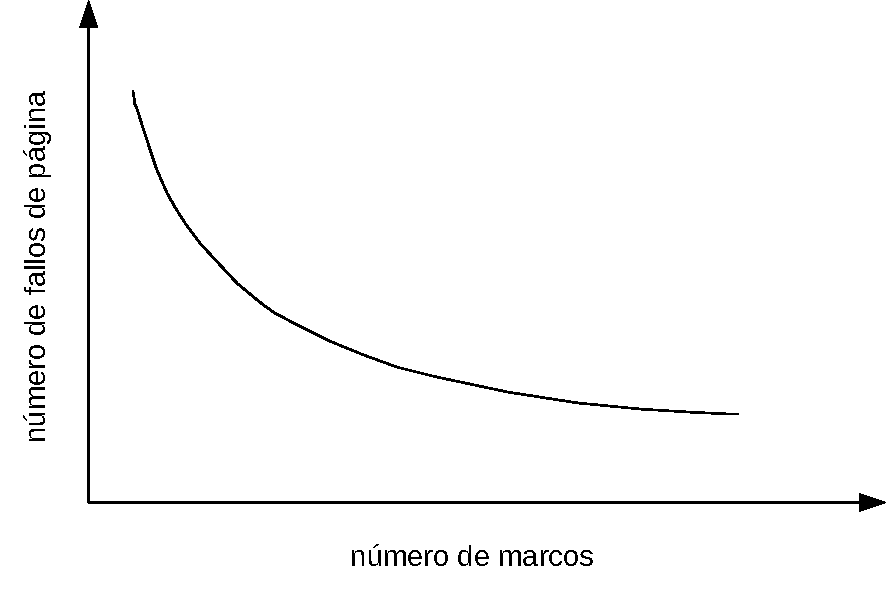
\includegraphics[width=0.8\textwidth]{media/C17_memoria_virtual/fallos_de_página_frente_a_marcos.pdf}
\caption{Fallos de página frente a número de
marcos.}\label{fig-fallos-de-puxe1gina-frente-a-marcos}
\end{figure}

Es de esperar que si el número de marcos disponibles aumenta, el número
de \textbf{fallos de página} disminuya (véase la
\hyperref[fig-fallos-de-puxe1gina-frente-a-marcos]{Fallos de página
frente a número de marcos.}). Sin embargo, con el \textbf{algoritmo
FIFO} el número de \textbf{fallos de página} puede aumentar cuando el
número de marcos disponibles se incrementa. Es lo que se conoce como la
\textbf{{}anormalidad de Belady}.

\begin{figure}
\centering
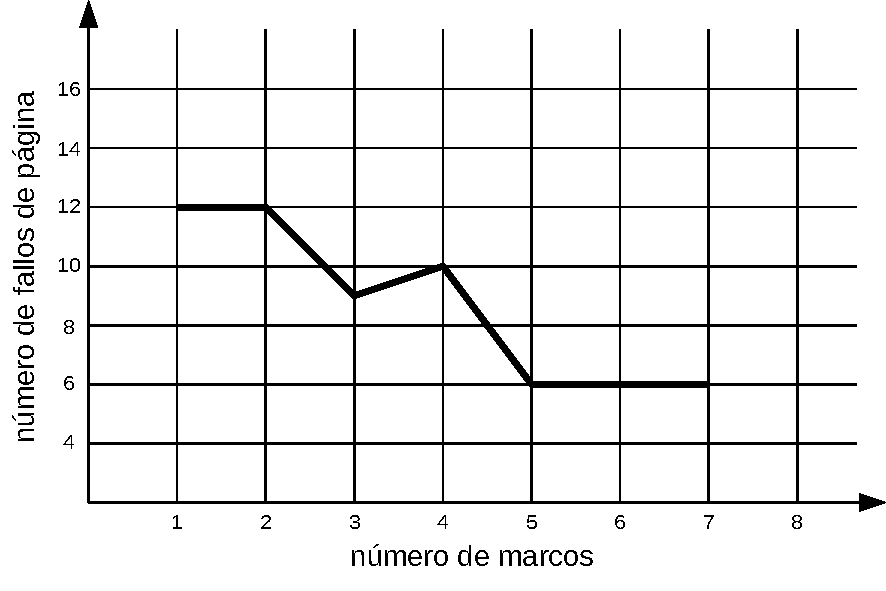
\includegraphics[width=0.8\textwidth]{media/C17_memoria_virtual/anormalidad_de_belady.pdf}
\caption{Fallos de página con el algoritmo de reemplazo
FIFO.}\label{fig-anormalidad-de-belady}
\end{figure}

Para ilustrarlo consideraremos la siguiente traza de referencias:

\begin{verbatim}
1, 2, 3, 4, 1, 2, 5, 1, 2, 3, 4, 5
\end{verbatim}

La \hyperref[fig-anormalidad-de-belady]{Fallos de página con el
algoritmo de reemplazo FIFO.} muestra la curva de \textbf{fallos de
página} frente el número de marcos. Como se puede apreciar, el número de
\textbf{fallos de página} con cuatro marcos es superior al número de
fallos con tres marcos, aunque era de esperar que el número de fallos de
páginas decrementara al aumentar el número de marcos.

\subsubsection{Reemplazo óptimo}\label{_reemplazo_uxf3ptimo}

{} {} Como resultado del descubrimiento de la \textbf{anormalidad de
Belady} se comenzó a buscar un algoritmo de reemplazo de página óptimo.
Es decir:

\begin{itemize}
\item
  Que tuviera la \textbf{tasa de fallo de página} más baja posible.
\item
  Que nunca sufra de la \textbf{anormalidad de Belady}.
\end{itemize}

Ese algoritmo existe y consiste en reemplazar la página que no va a ser
utilizada en el mayor periodo de tiempo.

\begin{longtable}[]{@{}
  >{\raggedright\arraybackslash}p{(\linewidth - 38\tabcolsep) * \real{0.0500}}
  >{\raggedright\arraybackslash}p{(\linewidth - 38\tabcolsep) * \real{0.0500}}
  >{\raggedright\arraybackslash}p{(\linewidth - 38\tabcolsep) * \real{0.0500}}
  >{\raggedright\arraybackslash}p{(\linewidth - 38\tabcolsep) * \real{0.0500}}
  >{\raggedright\arraybackslash}p{(\linewidth - 38\tabcolsep) * \real{0.0500}}
  >{\raggedright\arraybackslash}p{(\linewidth - 38\tabcolsep) * \real{0.0500}}
  >{\raggedright\arraybackslash}p{(\linewidth - 38\tabcolsep) * \real{0.0500}}
  >{\raggedright\arraybackslash}p{(\linewidth - 38\tabcolsep) * \real{0.0500}}
  >{\raggedright\arraybackslash}p{(\linewidth - 38\tabcolsep) * \real{0.0500}}
  >{\raggedright\arraybackslash}p{(\linewidth - 38\tabcolsep) * \real{0.0500}}
  >{\raggedright\arraybackslash}p{(\linewidth - 38\tabcolsep) * \real{0.0500}}
  >{\raggedright\arraybackslash}p{(\linewidth - 38\tabcolsep) * \real{0.0500}}
  >{\raggedright\arraybackslash}p{(\linewidth - 38\tabcolsep) * \real{0.0500}}
  >{\raggedright\arraybackslash}p{(\linewidth - 38\tabcolsep) * \real{0.0500}}
  >{\raggedright\arraybackslash}p{(\linewidth - 38\tabcolsep) * \real{0.0500}}
  >{\raggedright\arraybackslash}p{(\linewidth - 38\tabcolsep) * \real{0.0500}}
  >{\raggedright\arraybackslash}p{(\linewidth - 38\tabcolsep) * \real{0.0500}}
  >{\raggedright\arraybackslash}p{(\linewidth - 38\tabcolsep) * \real{0.0500}}
  >{\raggedright\arraybackslash}p{(\linewidth - 38\tabcolsep) * \real{0.0500}}
  >{\raggedright\arraybackslash}p{(\linewidth - 38\tabcolsep) * \real{0.0500}}@{}}
\toprule
\begin{minipage}[b]{\linewidth}\centering
7
\end{minipage} & \begin{minipage}[b]{\linewidth}\centering
0
\end{minipage} & \begin{minipage}[b]{\linewidth}\centering
1
\end{minipage} & \begin{minipage}[b]{\linewidth}\centering
2
\end{minipage} & \begin{minipage}[b]{\linewidth}\centering
0
\end{minipage} & \begin{minipage}[b]{\linewidth}\centering
2
\end{minipage} & \begin{minipage}[b]{\linewidth}\centering
0
\end{minipage} & \begin{minipage}[b]{\linewidth}\centering
2
\end{minipage} & \begin{minipage}[b]{\linewidth}\centering
4
\end{minipage} & \begin{minipage}[b]{\linewidth}\centering
0
\end{minipage} & \begin{minipage}[b]{\linewidth}\centering
2
\end{minipage} & \begin{minipage}[b]{\linewidth}\centering
0
\end{minipage} & \begin{minipage}[b]{\linewidth}\centering
1
\end{minipage} & \begin{minipage}[b]{\linewidth}\centering
3
\end{minipage} & \begin{minipage}[b]{\linewidth}\centering
0
\end{minipage} & \begin{minipage}[b]{\linewidth}\centering
1
\end{minipage} & \begin{minipage}[b]{\linewidth}\centering
2
\end{minipage} & \begin{minipage}[b]{\linewidth}\centering
7
\end{minipage} & \begin{minipage}[b]{\linewidth}\centering
0
\end{minipage} & \begin{minipage}[b]{\linewidth}\centering
1
\end{minipage} \\
\midrule
\endhead
\bottomrule
\endlastfoot
7 & 7 & 7 & 2 & & & & & 2 & & & & 2 & 3 & & & 2 & 2 & & \\
& 0 & 0 & 0 & & & & & 0 & & & & 0 & 0 & & & 0 & 0 & & \\
& & 1 & 1 & & & & & 4 & & & & 1 & 1 & & & 1 & 7 & & \\
\textbf{F} & \textbf{F} & \textbf{F} & \textbf{F} & & & & & \textbf{F} & & & & \textbf{F} & \textbf{F} & & & \textbf{F} & \textbf{F} & & \\
\multicolumn{20}{c}{\textbf{9 fallos de página}} \\
\end{longtable}
\par\vspace{0pt}

Desafortunadamente, el \textbf{algoritmo de reemplazo óptimo} es difícil
de implementar, puesto que necesita saber las páginas que serán
referenciadas en el futuro. Por lo que solo se usa en estudios
comparativos, con el fin de saber cuánto se aproxima al óptimo un
algoritmo de reemplazo determinado.

\subsubsection{Reemplazo LRU}\label{_reemplazo_lru}

{} {} El \textbf{algoritmo de reemplazo de página {}LRU} (\emph{Least
Recently Used}) es una aproximación del óptimo. La hipótesis es que si
una página no ha sido usada durante un gran periodo de tiempo, entonces
probablemente tampoco será utilizada en el futuro; por lo que
reemplazando la página que hace más tiempo que no se usa, nos estaríamos
aproximando al algoritmo óptimo. Vamos a ilustrarlo con un ejemplo:

\begin{longtable}[]{@{}
  >{\raggedright\arraybackslash}p{(\linewidth - 38\tabcolsep) * \real{0.0500}}
  >{\raggedright\arraybackslash}p{(\linewidth - 38\tabcolsep) * \real{0.0500}}
  >{\raggedright\arraybackslash}p{(\linewidth - 38\tabcolsep) * \real{0.0500}}
  >{\raggedright\arraybackslash}p{(\linewidth - 38\tabcolsep) * \real{0.0500}}
  >{\raggedright\arraybackslash}p{(\linewidth - 38\tabcolsep) * \real{0.0500}}
  >{\raggedright\arraybackslash}p{(\linewidth - 38\tabcolsep) * \real{0.0500}}
  >{\raggedright\arraybackslash}p{(\linewidth - 38\tabcolsep) * \real{0.0500}}
  >{\raggedright\arraybackslash}p{(\linewidth - 38\tabcolsep) * \real{0.0500}}
  >{\raggedright\arraybackslash}p{(\linewidth - 38\tabcolsep) * \real{0.0500}}
  >{\raggedright\arraybackslash}p{(\linewidth - 38\tabcolsep) * \real{0.0500}}
  >{\raggedright\arraybackslash}p{(\linewidth - 38\tabcolsep) * \real{0.0500}}
  >{\raggedright\arraybackslash}p{(\linewidth - 38\tabcolsep) * \real{0.0500}}
  >{\raggedright\arraybackslash}p{(\linewidth - 38\tabcolsep) * \real{0.0500}}
  >{\raggedright\arraybackslash}p{(\linewidth - 38\tabcolsep) * \real{0.0500}}
  >{\raggedright\arraybackslash}p{(\linewidth - 38\tabcolsep) * \real{0.0500}}
  >{\raggedright\arraybackslash}p{(\linewidth - 38\tabcolsep) * \real{0.0500}}
  >{\raggedright\arraybackslash}p{(\linewidth - 38\tabcolsep) * \real{0.0500}}
  >{\raggedright\arraybackslash}p{(\linewidth - 38\tabcolsep) * \real{0.0500}}
  >{\raggedright\arraybackslash}p{(\linewidth - 38\tabcolsep) * \real{0.0500}}
  >{\raggedright\arraybackslash}p{(\linewidth - 38\tabcolsep) * \real{0.0500}}@{}}
\toprule\noalign{}
\begin{minipage}[b]{\linewidth}\centering
7
\end{minipage} & \begin{minipage}[b]{\linewidth}\centering
0
\end{minipage} & \begin{minipage}[b]{\linewidth}\centering
1
\end{minipage} & \begin{minipage}[b]{\linewidth}\centering
2
\end{minipage} & \begin{minipage}[b]{\linewidth}\centering
0
\end{minipage} & \begin{minipage}[b]{\linewidth}\centering
2
\end{minipage} & \begin{minipage}[b]{\linewidth}\centering
0
\end{minipage} & \begin{minipage}[b]{\linewidth}\centering
2
\end{minipage} & \begin{minipage}[b]{\linewidth}\centering
4
\end{minipage} & \begin{minipage}[b]{\linewidth}\centering
0
\end{minipage} & \begin{minipage}[b]{\linewidth}\centering
2
\end{minipage} & \begin{minipage}[b]{\linewidth}\centering
0
\end{minipage} & \begin{minipage}[b]{\linewidth}\centering
1
\end{minipage} & \begin{minipage}[b]{\linewidth}\centering
3
\end{minipage} & \begin{minipage}[b]{\linewidth}\centering
0
\end{minipage} & \begin{minipage}[b]{\linewidth}\centering
1
\end{minipage} & \begin{minipage}[b]{\linewidth}\centering
2
\end{minipage} & \begin{minipage}[b]{\linewidth}\centering
7
\end{minipage} & \begin{minipage}[b]{\linewidth}\centering
0
\end{minipage} & \begin{minipage}[b]{\linewidth}\centering
1
\end{minipage} \\
\midrule\noalign{}
\endhead
\bottomrule\noalign{}
\endlastfoot
7 & 7 & 7 & 2 & & & & & 2 & & & & 2 & 3 & & & 2 & 2 & 2 & 1 \\
& 0 & 0 & 0 & & & & & 0 & & & & 0 & 0 & & & 0 & 7 & 7 & 7 \\
& & 1 & 1 & & & & & 4 & & & & 1 & 1 & & & 1 & 1 & 0 & 0 \\
\textbf{F} & \textbf{F} & \textbf{F} & \textbf{F} & & & & & \textbf{F} & & & & \textbf{F} & \textbf{F} & & & \textbf{F} & \textbf{F} & \textbf{F} & \textbf{F} \\
\multicolumn{20}{c}{\textbf{11 fallos de página}} \\
\end{longtable}

Este algoritmo se considera bastante eficiente cuando se aplica al
reemplazo de páginas, por lo que es utilizado con frecuencia.

Un detalle significativo es que necesita asociar cada página con el
momento en que fue utilizada por última vez. Aunque se pueden utilizar
interrupciones para implementarlo por software ---monitorizando cada
acceso a la memoria--- esta solución es muy ineficiente, puesto que se
necesitaría actualizar algunos datos en la memoria en cada referencia a
una página. Por ello el reemplazo LRU es inconcebible sin apoyo del
hardware.

Son posibles dos implementaciones:

\begin{itemize}
\item
  Utilizando contadores:

  \begin{enumerate}
  \def\labelenumi{\arabic{enumi}.}
  \item
    La CPU debe tener un reloj lógico o contador que se incrementa con
    cada referencia a la memoria.
  \item
    A cada página se añade un campo de \textbf{instante de uso}, que se
    almacena en la entrada de la tabla de páginas correspondiente.
  \item
    Cuando una página es referenciada, el valor del contador de la CPU
    se almacena en el campo de \textbf{instante de uso} de dicha página.
  \end{enumerate}

  Esta implementación requiere que se haga una escritura en la memoria
  con cada referencia. Además de una búsqueda por toda la tabla de
  páginas para localizar la página LRU.
\item
  Utilizando una pila:

  \begin{enumerate}
  \def\labelenumi{\arabic{enumi}.}
  \item
    Se utiliza una pila de números de página.
  \item
    Si se referencia una página, se quita el número correspondiente de
    la mitad de la pila y se inserta arriba. Debido a esto, lo mejor es
    implementarla como una lista doblemente enlazada.
  \end{enumerate}
\item
  La actualización de la pila ---que debe realizarse en cada
  referencia--- tiene mayor coste que en la implementación anterior,
  pues puede ser necesario cambiar hasta 6 punteros. Sin embargo, no es
  necesario realizar ninguna búsqueda para seleccionar la víctima del
  reemplazo, puesto que esta se puede extraer directamente del final de
  la pila.
\item
  Es una estrategia ideal para ser implementada en software o
  microcódigo.
\end{itemize}

El \textbf{algoritmo reemplazo LRU} pertenece a una clase denominada
\textbf{algoritmos de pila}, que nunca se ven afectados por la
\textbf{anormalidad de Belady}. En estos algoritmos, las páginas en
memoria en un instante dado para \emph{N} marcos son un subconjunto de
las que podría haber con \emph{N} + 1 marcos. Concretamente, en el
\textbf{algoritmo LRU} las páginas en los marcos son las \emph{N}
páginas más referenciadas recientemente. Si el número de marcos
aumentase, estas \emph{N} páginas seguirán estando en memoria, pues
siguen siendo las referenciadas más recientemente.

\subsubsection{Reemplazo LRU
aproximado}\label{_reemplazo_lru_aproximado}

Pocos sistemas tienen soporte para utilizar el \textbf{algoritmo de
reemplazo de página LRU}. Incluso en algunos casos no hay soporte de
ningún tipo, por lo que no queda más remedio que utilizar el reemplazo
FIFO.

Sin embargo, muchos proporcionan algo de ayuda en la forma de un
\textbf{bit de referencia}{}:

\begin{itemize}
\item
  Cada entrada de la tabla de páginas tiene un \textbf{bit de
  referencia}.
\item
  El hardware pone a 1 el \textbf{bit de referencia} cada vez que se
  referencia a una página.
\end{itemize}

Con el \textbf{bit de referencia} no podemos saber con exactitud el
instante, pero sí que una página ha sido referenciada recientemente.
Utilizándolo, podemos implementar diversas aproximaciones al algoritmo
LRU.

\paragraph{Reemplazo NRU}\label{_reemplazo_nru}

{} {} En el \textbf{algoritmo de reemplazo de página {}NRU} se utiliza
el \textbf{bit de referencia} de la siguiente manera:

\begin{enumerate}
\def\labelenumi{\arabic{enumi}.}
\item
  En intervalos regulares de tiempo, todos los \textbf{bits de
  referencia} son puestos a cero por el sistema operativo.
\item
  Según los procesos se van ejecutando, el \textbf{bit de referencia}
  asociado a cada página se pone a 1 por el hardware, al ser
  referenciadas.
\item
  Cuando haya que escoger una página para ser reemplazada, se intenta
  seleccionar una que no haya sido referenciada ---es decir, con el bit
  de referencia a 0---.
\item
  En caso de que haya varias alternativas entre las que elegir se puede
  utilizar el \textbf{algoritmo de reemplazo de página FIFO} o escoger
  un aleatoriamente.
\end{enumerate}

Vamos a ilustrarlo con un ejemplo:

\begin{itemize}
\item
  Utilizaremos 3 marcos de página.
\item
  Indicaremos el valor del bit de referencia con un superíndice junto al
  número de página.
\end{itemize}

No debemos olvidar que en caso de que ocurra un fallo de página, después
de la carga de la página se reinicia la instrucción que generó dicho
fallo. Por lo tanto, habrá un acceso que pondrá el \textbf{bit de
referencia a 1}.

\begin{itemize}
\item
  Marcaremos con una flecha el instante de tiempo en el que todos los
  bits de referencia se ponen a cero.
\end{itemize}

En un sistema operativo real los bits son desplazados en intervalos
fijos de tiempo. Pero esto no tiene que coincidir con una cantidad fija
de referencias en la traza, puesto que hemos eliminado las referencias
consecutivas a una misma página.

\begin{itemize}
\item
  En caso de coincidencia, utilizaremos el \textbf{reemplazo FIFO} para
  seleccionar la víctima.
\end{itemize}

\begin{longtable}[]{@{}
  >{\raggedright\arraybackslash}p{(\linewidth - 38\tabcolsep) * \real{0.0500}}
  >{\raggedright\arraybackslash}p{(\linewidth - 38\tabcolsep) * \real{0.0500}}
  >{\raggedright\arraybackslash}p{(\linewidth - 38\tabcolsep) * \real{0.0500}}
  >{\raggedright\arraybackslash}p{(\linewidth - 38\tabcolsep) * \real{0.0500}}
  >{\raggedright\arraybackslash}p{(\linewidth - 38\tabcolsep) * \real{0.0500}}
  >{\raggedright\arraybackslash}p{(\linewidth - 38\tabcolsep) * \real{0.0500}}
  >{\raggedright\arraybackslash}p{(\linewidth - 38\tabcolsep) * \real{0.0500}}
  >{\raggedright\arraybackslash}p{(\linewidth - 38\tabcolsep) * \real{0.0500}}
  >{\raggedright\arraybackslash}p{(\linewidth - 38\tabcolsep) * \real{0.0500}}
  >{\raggedright\arraybackslash}p{(\linewidth - 38\tabcolsep) * \real{0.0500}}
  >{\raggedright\arraybackslash}p{(\linewidth - 38\tabcolsep) * \real{0.0500}}
  >{\raggedright\arraybackslash}p{(\linewidth - 38\tabcolsep) * \real{0.0500}}
  >{\raggedright\arraybackslash}p{(\linewidth - 38\tabcolsep) * \real{0.0500}}
  >{\raggedright\arraybackslash}p{(\linewidth - 38\tabcolsep) * \real{0.0500}}
  >{\raggedright\arraybackslash}p{(\linewidth - 38\tabcolsep) * \real{0.0500}}
  >{\raggedright\arraybackslash}p{(\linewidth - 38\tabcolsep) * \real{0.0500}}
  >{\raggedright\arraybackslash}p{(\linewidth - 38\tabcolsep) * \real{0.0500}}
  >{\raggedright\arraybackslash}p{(\linewidth - 38\tabcolsep) * \real{0.0500}}
  >{\raggedright\arraybackslash}p{(\linewidth - 38\tabcolsep) * \real{0.0500}}
  >{\raggedright\arraybackslash}p{(\linewidth - 38\tabcolsep) * \real{0.0500}}@{}}
\toprule
\endhead
\bottomrule
\endlastfoot
& & & & \textbf{↓} & & & \textbf{↓} & & & \textbf{↓} & & & & \textbf{↓} & & & \textbf{↓} & & \\
\textbf{7} & \textbf{0} & \textbf{1} & \textbf{2} & \textbf{0} & \textbf{2} & \textbf{0} & \textbf{2} & \textbf{4} & \textbf{0} & \textbf{2} & \textbf{0} & \textbf{1} & \textbf{3} & \textbf{0} & \textbf{1} & \textbf{2} & \textbf{7} & \textbf{0} & \textbf{1} \\
7\textsuperscript{1} & 7\textsuperscript{1} & 7\textsuperscript{1} & 2\textsuperscript{1} & 2\textsuperscript{0} & 2\textsuperscript{1} & & 2\textsuperscript{1} & 2\textsuperscript{1} & 2\textsuperscript{1} & 2\textsuperscript{1} & 2\textsuperscript{1} & 2\textsuperscript{1} & 3\textsuperscript{1} & 3\textsuperscript{0} & 3\textsuperscript{0} & 2\textsuperscript{1} & 2\textsuperscript{0} & 2\textsuperscript{0} & 2\textsuperscript{0} \\
& 0\textsuperscript{1} & 0\textsuperscript{1} & 0\textsuperscript{1} & 0\textsuperscript{1} & 0\textsuperscript{1} & & 0\textsuperscript{0} & 4\textsuperscript{1} & 4\textsuperscript{1} & 4\textsuperscript{0} & 4\textsuperscript{0} & 1\textsuperscript{1} & 1\textsuperscript{1} & 1\textsuperscript{0} & 1\textsuperscript{1} & 1\textsuperscript{1} & 7\textsuperscript{1} & 7\textsuperscript{1} & 7\textsuperscript{1} \\
& & 1\textsuperscript{1} & 1\textsuperscript{1} & 1\textsuperscript{0} & 1\textsuperscript{0} & & 1\textsuperscript{0} & 1\textsuperscript{0} & 0\textsuperscript{1} & 0\textsuperscript{0} & 0\textsuperscript{1} & 0\textsuperscript{1} & 0\textsuperscript{1} & 0\textsuperscript{1} & 0\textsuperscript{1} & 0\textsuperscript{1} & 0\textsuperscript{0} & 0\textsuperscript{1} & 1\textsuperscript{1} \\
\textbf{F} & \textbf{F} & \textbf{F} & \textbf{F} & & & & & \textbf{F} & \textbf{F} & & & \textbf{F} & \textbf{F} & & & \textbf{F} & \textbf{F} & & \textbf{F} \\
\multicolumn{20}{c}{\textbf{11 fallos de página}} \\
\end{longtable}
\par\vspace{0pt}

Se puede mejorar el algoritmo anterior considerando tanto el \textbf{bit
de referencia} como el \textbf{bit de modificado}, para clasificar las
páginas en distintas categorías y escoger una página en la mejor
categoría. Este es el tipo más común de \textbf{algoritmo de reemplazo
de página NRU}, pero lo veremos en el
\hyperref[_algoritmo_de_la_segunda_oportunidad_mejorado]{Algoritmo de la
segunda oportunidad mejorado} bajo el nombre de \textbf{Algoritmo de la
segunda oportunidad mejorado}.

\paragraph{Con bits de referencia
adicionales}\label{_con_bits_de_referencia_adicionales}

Podemos obtener información adicional sobre el orden en que se realizan
las referencias, guardando los \textbf{bits de referencia} en intervalos
periódicos de tiempo. El \textbf{reemplazo LRU aproximado con bits de
referencia adicionales}, o de \textbf{envejecimiento}, consiste en lo
siguiente:

\begin{enumerate}
\def\labelenumi{\arabic{enumi}.}
\item
  Aparte del \textbf{bit de referencia}, cada página tiene un conjunto
  de \textbf{bits de referencia adicionales} ---por ejemplo, 8 bits---
  que se guardan en alguna tabla interna que mantiene el sistema
  operativo.
\item
  A intervalos regulares ---por ejemplo, cada 100 ms--- el sistema
  operativo desplaza los \textbf{bits de referencia adicionales} de cada
  página; insertando el \textbf{bit de referencia} de la página en el
  bit de orden más alto y descartando el bit de orden más bajo.
\item
  Cuando haya que escoger una página para ser reemplazada se escoge la
  que tenga el valor más pequeño en el conjunto de \textbf{bits de
  referencia adicionales}. Esto es así, puesto que dicho conjunto
  contiene la historia de referencias de la página. Por ejemplo, \{1 1 0
  0 0 1 0 0\} es más reciente que \{0 1 1 1 0 1 1 1\}.
\item
  Se puede utilizar el \textbf{algoritmo de reemplazo de página FIFO} o
  escoger un aleatoriamente, si dos páginas tienen el mismo valor.
\end{enumerate}

Vamos a ilustrarlo con un ejemplo:

\begin{itemize}
\item
  Utilizaremos 3 marcos de página.
\item
  Utilizaremos 2 bits adicionales.
\item
  Indicaremos el valor del \textbf{bit de referencia} y de los
  \textbf{bits adicionales} con un superíndice junto al número de
  página.
\item
  Marcaremos con una flecha el instante de tiempo en el que los bits son
  desplazados por el sistema operativo.
\item
  En caso de coincidencia, utilizaremos el \textbf{reemplazo FIFO} para
  seleccionar la víctima.
\end{itemize}

\begin{longtable}[]{@{}
  >{\raggedright\arraybackslash}p{(\linewidth - 38\tabcolsep) * \real{0.0500}}
  >{\raggedright\arraybackslash}p{(\linewidth - 38\tabcolsep) * \real{0.0500}}
  >{\raggedright\arraybackslash}p{(\linewidth - 38\tabcolsep) * \real{0.0500}}
  >{\raggedright\arraybackslash}p{(\linewidth - 38\tabcolsep) * \real{0.0500}}
  >{\raggedright\arraybackslash}p{(\linewidth - 38\tabcolsep) * \real{0.0500}}
  >{\raggedright\arraybackslash}p{(\linewidth - 38\tabcolsep) * \real{0.0500}}
  >{\raggedright\arraybackslash}p{(\linewidth - 38\tabcolsep) * \real{0.0500}}
  >{\raggedright\arraybackslash}p{(\linewidth - 38\tabcolsep) * \real{0.0500}}
  >{\raggedright\arraybackslash}p{(\linewidth - 38\tabcolsep) * \real{0.0500}}
  >{\raggedright\arraybackslash}p{(\linewidth - 38\tabcolsep) * \real{0.0500}}
  >{\raggedright\arraybackslash}p{(\linewidth - 38\tabcolsep) * \real{0.0500}}
  >{\raggedright\arraybackslash}p{(\linewidth - 38\tabcolsep) * \real{0.0500}}
  >{\raggedright\arraybackslash}p{(\linewidth - 38\tabcolsep) * \real{0.0500}}
  >{\raggedright\arraybackslash}p{(\linewidth - 38\tabcolsep) * \real{0.0500}}
  >{\raggedright\arraybackslash}p{(\linewidth - 38\tabcolsep) * \real{0.0500}}
  >{\raggedright\arraybackslash}p{(\linewidth - 38\tabcolsep) * \real{0.0500}}
  >{\raggedright\arraybackslash}p{(\linewidth - 38\tabcolsep) * \real{0.0500}}
  >{\raggedright\arraybackslash}p{(\linewidth - 38\tabcolsep) * \real{0.0500}}
  >{\raggedright\arraybackslash}p{(\linewidth - 38\tabcolsep) * \real{0.0500}}
  >{\raggedright\arraybackslash}p{(\linewidth - 38\tabcolsep) * \real{0.0500}}@{}}
\toprule
\endhead
\bottomrule
\endlastfoot
& & & & \textbf{↓} & & & \textbf{↓} & & & \textbf{↓} & & & & \textbf{↓} & & & \textbf{↓} & & \\
\textbf{7} & \textbf{0} & \textbf{1} & \textbf{2} & \textbf{0} & \textbf{2} & \textbf{0} & \textbf{2} & \textbf{4} & \textbf{0} & \textbf{2} & \textbf{0} & \textbf{1} & \textbf{3} & \textbf{0} & \textbf{1} & \textbf{2} & \textbf{7} & \textbf{0} & \textbf{1} \\
7\textsuperscript{1|00} & 7\textsuperscript{1|00} & 7\textsuperscript{1|00} & 2\textsuperscript{1|00} & 2\textsuperscript{0|10} & 2\textsuperscript{1|10} & 2\textsuperscript{1|10} & 2\textsuperscript{1|11} & 2\textsuperscript{1|11} & 2\textsuperscript{1|11} & 2\textsuperscript{1|11} & 2\textsuperscript{1|11} & 2\textsuperscript{1|11} & 2\textsuperscript{1|11} & 2\textsuperscript{0|11} & 2\textsuperscript{0|11} & 2\textsuperscript{1|11} & 2\textsuperscript{0|11} & 2\textsuperscript{0|11} & 2\textsuperscript{0|11} \\
& 0\textsuperscript{1|00} & 0\textsuperscript{1|00} & 0\textsuperscript{1|00} & 0\textsuperscript{1|10} & 0\textsuperscript{1|10} & 0\textsuperscript{1|10} & 0\textsuperscript{0|11} & 0\textsuperscript{0|11} & 0\textsuperscript{1|11} & 0\textsuperscript{0|11} & 0\textsuperscript{1|11} & 0\textsuperscript{1|11} & 0\textsuperscript{1|11} & 0\textsuperscript{1|11} & 0\textsuperscript{1|11} & 0\textsuperscript{1|11} & 0\textsuperscript{0|11} & 0\textsuperscript{1|11} & 0\textsuperscript{1|11} \\
& & 1\textsuperscript{1|00} & 1\textsuperscript{1|00} & 1\textsuperscript{0|10} & 1\textsuperscript{0|10} & 1\textsuperscript{0|10} & 1\textsuperscript{0|01} & 4\textsuperscript{1|00} & 4\textsuperscript{1|00} & 4\textsuperscript{0|10} & 4\textsuperscript{0|10} & 1\textsuperscript{1|00} & 3\textsuperscript{1|00} & 3\textsuperscript{0|10} & 1\textsuperscript{1|00} & 1\textsuperscript{1|00} & 7\textsuperscript{1|00} & 7\textsuperscript{1|00} & 1\textsuperscript{1|00} \\
\textbf{F} & \textbf{F} & \textbf{F} & \textbf{F} & & & & & \textbf{F} & & & & \textbf{F} & \textbf{F} & & \textbf{F} & & \textbf{F} & & \textbf{F} \\
\multicolumn{20}{c}{\textbf{10 fallos de página}} \\
\end{longtable}
\par\vspace{0pt}

El número de \textbf{bits adicionales} puede variar de una
implementación a otra, pero en cualquier caso debe ser seleccionado para
realizar la actualización lo más rápidamente posible, teniendo en cuenta
las características del hardware. En un caso extremo, el número de
\textbf{bits de referencia adicionales} podría ser cero, dejando solo el
\textbf{bit de referencia}. A este algoritmo se lo conoce como el
\textbf{algoritmo de la segunda oportunidad}.

\paragraph{Algoritmo de la segunda
oportunidad}\label{_algoritmo_de_la_segunda_oportunidad}

{} {} {} {} {} El \textbf{algoritmo de reemplazo de la segunda
oportunidad} o del \textbf{reloj} es un \textbf{algoritmo de reemplazo
de página FIFO}, pero donde una página es seleccionada considerando el
\textbf{bit de referencia}:

\begin{enumerate}
\def\labelenumi{\arabic{enumi}.}
\item
  Cuando es necesario seleccionar una víctima para reemplazo se extrae
  una página de la cola FIFO. Esta cola contiene todas las páginas con
  marcos asignados y en el orden en que fueron cargadas, como ocurre con
  el \textbf{algoritmo FIFO de reemplazo}.
\item
  Si el \textbf{bit de referencia} está a 0, se utiliza esta página para
  reemplazo.
\item
  Si el \textbf{bit de referencia} está a 1:

  \begin{enumerate}
  \def\labelenumii{\alph{enumii}.}
  \item
    Se pone el \textbf{bit de referencia} a 0 y se vuelve a insertar la
    página en el final de la cola.
  \item
    Se extrae la siguiente página del principio de la cola y se vuelve
    al punto 2.
  \end{enumerate}
\end{enumerate}

De este esquema podemos destacar algunos aspectos:

\begin{itemize}
\item
  Una página a la que se le da la segunda oportunidad, no será
  reemplazada hasta que no se le dé la segunda oportunidad a todas las
  demás; siempre que no sea referenciada antes y el \textbf{bit de
  referencia} se vuelva a poner a 1.
\item
  En el peor de los casos, cuando todas las páginas tienen sus bits a
  uno, degenera en un reemplazo FIFO.
\end{itemize}

Vamos a ilustrarlo con un ejemplo:

\begin{itemize}
\item
  Utilizaremos 3 marcos de página.
\item
  Indicaremos el valor del \textbf{bit de referencia} con un superíndice
  junto al número de página en el marco.
\item
  Indicaremos el principio de la cola con una flecha junto al número de
  página.
\end{itemize}

\begin{longtable}[]{@{}
  >{\raggedright\arraybackslash}p{(\linewidth - 38\tabcolsep) * \real{0.0500}}
  >{\raggedright\arraybackslash}p{(\linewidth - 38\tabcolsep) * \real{0.0500}}
  >{\raggedright\arraybackslash}p{(\linewidth - 38\tabcolsep) * \real{0.0500}}
  >{\raggedright\arraybackslash}p{(\linewidth - 38\tabcolsep) * \real{0.0500}}
  >{\raggedright\arraybackslash}p{(\linewidth - 38\tabcolsep) * \real{0.0500}}
  >{\raggedright\arraybackslash}p{(\linewidth - 38\tabcolsep) * \real{0.0500}}
  >{\raggedright\arraybackslash}p{(\linewidth - 38\tabcolsep) * \real{0.0500}}
  >{\raggedright\arraybackslash}p{(\linewidth - 38\tabcolsep) * \real{0.0500}}
  >{\raggedright\arraybackslash}p{(\linewidth - 38\tabcolsep) * \real{0.0500}}
  >{\raggedright\arraybackslash}p{(\linewidth - 38\tabcolsep) * \real{0.0500}}
  >{\raggedright\arraybackslash}p{(\linewidth - 38\tabcolsep) * \real{0.0500}}
  >{\raggedright\arraybackslash}p{(\linewidth - 38\tabcolsep) * \real{0.0500}}
  >{\raggedright\arraybackslash}p{(\linewidth - 38\tabcolsep) * \real{0.0500}}
  >{\raggedright\arraybackslash}p{(\linewidth - 38\tabcolsep) * \real{0.0500}}
  >{\raggedright\arraybackslash}p{(\linewidth - 38\tabcolsep) * \real{0.0500}}
  >{\raggedright\arraybackslash}p{(\linewidth - 38\tabcolsep) * \real{0.0500}}
  >{\raggedright\arraybackslash}p{(\linewidth - 38\tabcolsep) * \real{0.0500}}
  >{\raggedright\arraybackslash}p{(\linewidth - 38\tabcolsep) * \real{0.0500}}
  >{\raggedright\arraybackslash}p{(\linewidth - 38\tabcolsep) * \real{0.0500}}
  >{\raggedright\arraybackslash}p{(\linewidth - 38\tabcolsep) * \real{0.0500}}@{}}
\toprule
\begin{minipage}[b]{\linewidth}\centering
7
\end{minipage} & \begin{minipage}[b]{\linewidth}\centering
0
\end{minipage} & \begin{minipage}[b]{\linewidth}\centering
1
\end{minipage} & \begin{minipage}[b]{\linewidth}\centering
2
\end{minipage} & \begin{minipage}[b]{\linewidth}\centering
0
\end{minipage} & \begin{minipage}[b]{\linewidth}\centering
2
\end{minipage} & \begin{minipage}[b]{\linewidth}\centering
0
\end{minipage} & \begin{minipage}[b]{\linewidth}\centering
2
\end{minipage} & \begin{minipage}[b]{\linewidth}\centering
4
\end{minipage} & \begin{minipage}[b]{\linewidth}\centering
0
\end{minipage} & \begin{minipage}[b]{\linewidth}\centering
2
\end{minipage} & \begin{minipage}[b]{\linewidth}\centering
0
\end{minipage} & \begin{minipage}[b]{\linewidth}\centering
1
\end{minipage} & \begin{minipage}[b]{\linewidth}\centering
3
\end{minipage} & \begin{minipage}[b]{\linewidth}\centering
0
\end{minipage} & \begin{minipage}[b]{\linewidth}\centering
1
\end{minipage} & \begin{minipage}[b]{\linewidth}\centering
2
\end{minipage} & \begin{minipage}[b]{\linewidth}\centering
7
\end{minipage} & \begin{minipage}[b]{\linewidth}\centering
0
\end{minipage} & \begin{minipage}[b]{\linewidth}\centering
1
\end{minipage} \\
\midrule
\endhead
\bottomrule
\endlastfoot
7\textsuperscript{1} & 7\textsuperscript{1} & →7\textsuperscript{1} & 2\textsuperscript{1} & 2\textsuperscript{0} & 2\textsuperscript{1} & & 2\textsuperscript{1} & →2\textsuperscript{1} & →2\textsuperscript{1} & →2\textsuperscript{1} & →2\textsuperscript{1} & 1\textsuperscript{1} & 1\textsuperscript{1} & →1\textsuperscript{1} & →1\textsuperscript{1} & 2\textsuperscript{1} & 2\textsuperscript{1} & 2\textsuperscript{1} & →2\textsuperscript{0} \\
→ & 0\textsuperscript{1} & 0\textsuperscript{1} & →0\textsuperscript{0} & →0\textsuperscript{1} & →0\textsuperscript{1} & & →0\textsuperscript{1} & 0\textsuperscript{0} & 0\textsuperscript{1} & 0\textsuperscript{1} & 0\textsuperscript{1} & →0\textsuperscript{0} & 3\textsuperscript{1} & 3\textsuperscript{1} & 3\textsuperscript{1} & →3\textsuperscript{0} & 7\textsuperscript{1} & 7\textsuperscript{1} & 7\textsuperscript{0} \\
& → & 1\textsuperscript{1} & 1\textsuperscript{0} & 1\textsuperscript{0} & 1\textsuperscript{0} & & 1\textsuperscript{0} & 4\textsuperscript{1} & 4\textsuperscript{1} & 4\textsuperscript{1} & 4\textsuperscript{1} & 4\textsuperscript{0} & →4\textsuperscript{0} & 0\textsuperscript{1} & 0\textsuperscript{1} & 0\textsuperscript{1} & →0\textsuperscript{1} & →0\textsuperscript{1} & 1\textsuperscript{1} \\
\textbf{F} & \textbf{F} & \textbf{F} & \textbf{F} & & & & & \textbf{F} & \textbf{F} & & & \textbf{F} & \textbf{F} & & & \textbf{F} & \textbf{F} & & \textbf{F} \\
\multicolumn{20}{c}{\textbf{11 fallos de página}} \\
\end{longtable}
\par\vspace{0pt}

\paragraph{Algoritmo de la segunda oportunidad
mejorado}\label{_algoritmo_de_la_segunda_oportunidad_mejorado}

Se puede mejorar el \textbf{algoritmo de la segunda oportunidad}
considerando tanto el \textbf{bit de referencia} como el \textbf{bit de
modificado}. Algunos autores denominan a este algoritmo como
\textbf{algoritmo de la segunda oportunidad mejorado}, mientras otro lo
llaman \textbf{{}NRU}, ya que es una versión mejorada del algoritmo del
\hyperref[_reemplazo_nru]{Reemplazo NRU}.

Con esos dos bits, el sistema operativo clasifica las páginas en una de
las siguientes cuatro clases:

\begin{enumerate}
\def\labelenumi{\arabic{enumi}.}
\item
  (0,0) ni recientemente usado ni modificado. Las páginas de esta clase
  son las mejores para ser reemplazadas.
\item
  (0,1) no usado recientemente pero modificado. No es una buena
  elección, puesto que hay que escribir primero la página al disco antes
  del reemplazo.
\item
  (1,0) recientemente usado pero no modificado. Probablemente será usada
  de nuevo en un corto espacio de tiempo.
\item
  (1,1) usada y modificada. Será utilizada pronto y la página tendría
  que ser escrita a disco para ser reemplazada.
\end{enumerate}

Cuando el reemplazo de página es invocado:

\begin{itemize}
\item
  Se examina la clase a la que pertenece cada página y se reemplaza una
  página en la clase de menor importancia que no esté vacía.
  Indudablemente, deberemos examinar la lista varias veces antes de
  encontrar la página que debe ser reemplazada.
\item
  A intervalos regulares los \textbf{bits de referencia} de todas las
  páginas son puestos a cero por el sistema operativo.
\end{itemize}

En un sistema real, el sistema operativo escribe las páginas modificadas
en el almacenamiento secundario cuando está desocupado y luego pone el
\textbf{bit de modificado} a 0.

Vamos a ilustrarlo con un ejemplo:

\begin{itemize}
\item
  Utilizaremos 3 marcos de página.
\item
  El que la referencia a la memoria sea para lectura \textbf{R} o
  escritura \textbf{W} vendrá indicado junto al número de página en la
  traza.
\item
  Marcaremos con una flecha el instante de tiempo en el que todos los
  bits de referencia se ponen a cero.
\item
  Indicaremos el valor del \textbf{bit de referencia} y del \textbf{bit
  de modificado} con un superíndice junto al número de página en el
  marco.
\item
  Indicaremos el principio de la cola con una flecha junto al número de
  página. Sirve para mantener un orden en las páginas, de tal forma que
  si hay varios candidatos de la misma categoría, se escoja el primero
  encontrado. Si, por ejemplo, la elección en caso de varios candidatos
  es aleatoria, no hace falta ese puntero.
\end{itemize}

\begin{longtable}[]{@{}
  >{\raggedright\arraybackslash}p{(\linewidth - 38\tabcolsep) * \real{0.0500}}
  >{\raggedright\arraybackslash}p{(\linewidth - 38\tabcolsep) * \real{0.0500}}
  >{\raggedright\arraybackslash}p{(\linewidth - 38\tabcolsep) * \real{0.0500}}
  >{\raggedright\arraybackslash}p{(\linewidth - 38\tabcolsep) * \real{0.0500}}
  >{\raggedright\arraybackslash}p{(\linewidth - 38\tabcolsep) * \real{0.0500}}
  >{\raggedright\arraybackslash}p{(\linewidth - 38\tabcolsep) * \real{0.0500}}
  >{\raggedright\arraybackslash}p{(\linewidth - 38\tabcolsep) * \real{0.0500}}
  >{\raggedright\arraybackslash}p{(\linewidth - 38\tabcolsep) * \real{0.0500}}
  >{\raggedright\arraybackslash}p{(\linewidth - 38\tabcolsep) * \real{0.0500}}
  >{\raggedright\arraybackslash}p{(\linewidth - 38\tabcolsep) * \real{0.0500}}
  >{\raggedright\arraybackslash}p{(\linewidth - 38\tabcolsep) * \real{0.0500}}
  >{\raggedright\arraybackslash}p{(\linewidth - 38\tabcolsep) * \real{0.0500}}
  >{\raggedright\arraybackslash}p{(\linewidth - 38\tabcolsep) * \real{0.0500}}
  >{\raggedright\arraybackslash}p{(\linewidth - 38\tabcolsep) * \real{0.0500}}
  >{\raggedright\arraybackslash}p{(\linewidth - 38\tabcolsep) * \real{0.0500}}
  >{\raggedright\arraybackslash}p{(\linewidth - 38\tabcolsep) * \real{0.0500}}
  >{\raggedright\arraybackslash}p{(\linewidth - 38\tabcolsep) * \real{0.0500}}
  >{\raggedright\arraybackslash}p{(\linewidth - 38\tabcolsep) * \real{0.0500}}
  >{\raggedright\arraybackslash}p{(\linewidth - 38\tabcolsep) * \real{0.0500}}
  >{\raggedright\arraybackslash}p{(\linewidth - 38\tabcolsep) * \real{0.0500}}@{}}
\toprule\noalign{}
\endhead
\bottomrule\noalign{}
\endlastfoot
& & & & \textbf{↓} & & & \textbf{↓} & & & \textbf{↓} & & & & \textbf{↓} & & & \textbf{↓} & & \\
\textbf{7r} & \textbf{0r} & \textbf{1w} & \textbf{2r} & \textbf{0r} & \textbf{2r} & \textbf{0w} & \textbf{2r} & \textbf{4w} & \textbf{0w} & \textbf{2r} & \textbf{0r} & \textbf{1r} & \textbf{3w} & \textbf{0r} & \textbf{1r} & \textbf{2w} & \textbf{7w} & \textbf{0r} & \textbf{1r} \\
7\textsuperscript{10} & 7\textsuperscript{10} & →7\textsuperscript{10} & 2\textsuperscript{10} & 2\textsuperscript{00} & 2\textsuperscript{10} & 2\textsuperscript{10} & 2\textsuperscript{10} & 2\textsuperscript{10} & →2\textsuperscript{10} & →2\textsuperscript{10} & →2\textsuperscript{10} & 2\textsuperscript{10} & 3\textsuperscript{11} & 3\textsuperscript{01} & 3\textsuperscript{01} & 2\textsuperscript{11} & 2\textsuperscript{01} & 2\textsuperscript{01} & 1\textsuperscript{10} \\
→ & 0\textsuperscript{10} & 0\textsuperscript{10} & →0\textsuperscript{10} & →0\textsuperscript{10} & →0\textsuperscript{10} & →0\textsuperscript{11} & →0\textsuperscript{01} & 4\textsuperscript{11} & 4\textsuperscript{11} & 4\textsuperscript{01} & 4\textsuperscript{01} & 1\textsuperscript{10} & →1\textsuperscript{10} & →1\textsuperscript{00} & →1\textsuperscript{10} & →1\textsuperscript{10} & 7\textsuperscript{11} & 7\textsuperscript{11} & →7\textsuperscript{11} \\
& → & 1\textsuperscript{11} & 1\textsuperscript{11} & 1\textsuperscript{01} & 1\textsuperscript{01} & 1\textsuperscript{01} & 1\textsuperscript{01} & →1\textsuperscript{01} & 0\textsuperscript{11} & 0\textsuperscript{01} & 0\textsuperscript{11} & →0\textsuperscript{11} & 0\textsuperscript{11} & 0\textsuperscript{11} & 0\textsuperscript{11} & 0\textsuperscript{11} & →0\textsuperscript{01} & →0\textsuperscript{11} & 0\textsuperscript{11} \\
\textbf{F} & \textbf{F} & \textbf{F} & \textbf{F} & & & & & \textbf{F} & \textbf{F} & & & \textbf{F} & \textbf{F} & & & \textbf{F} & \textbf{F} & & \textbf{F} \\
\multicolumn{20}{c}{\textbf{11 fallos de página}} \\
\end{longtable}

\subsubsection{Reemplazo basado en
contador}\label{_reemplazo_basado_en_contador}

Otros algoritmos utilizan un contador del número de referencias que son
realizadas a cada página. En esos casos, la elección de la víctima se
puede realizar utilizando dos esquemas: la que tiene el valor mayor o el
menor. Ninguno de los dos es muy común, ya que su implementación es
costosa y no son una buena aproximación del óptimo.

Por lo general, la actualización del contador no la realiza la CPU, ya
que leer la entrada de la página, incrementar el contador y volver a
guardar la entrada, tiene un coste importante. En su lugar:

\begin{enumerate}
\def\labelenumi{\arabic{enumi}.}
\item
  El contador de cada página se guarda en una tabla interna.
\item
  Periódicamente el sistema operativo examina el \textbf{bit de
  referencia} de cada página y si está a 1, incrementa el contador de la
  página correspondiente.
\end{enumerate}

El mayor problema es que permite hacer el seguimiento de la frecuencia
con la que se usan las páginas, pero no tiene en cuenta el periodo
durante el que se usan. Por ejemplo, los procesos durante su
inicialización pueden usar intensamente ciertas páginas y después no
necesitarlas más. Debido a que esas páginas han sido utilizadas
intensamente, tiene un contador de referencias con un valor muy alto,
por lo que son mantenidas en memoria aunque no vaya a ser utilizadas.

La solución es utilizar el \textbf{algoritmo LRU aproximado con bits de
referencia adicionales} (véase
\hyperref[_con_bits_de_referencia_adicionales]{Con bits de referencia
adicionales}) porque tiene un coste muy similar a este y prioriza las
usadas más recientemente sobre las que fueron usadas con mucha
frecuencia en el pasado.

\paragraph{Reemplazo LFU}\label{_reemplazo_lfu}

{} {} {} {} En el \textbf{algoritmo de reemplazo de página {}LFU}
(\emph{Least Frequently Used}) o \textbf{{}NFU} (\emph{Not Frequently
Used}) se escoge la página con el contador más bajo. Esto es así, puesto
que suponemos que las páginas menos referenciadas son las que no se
están utilizando de forma más activa.

Vamos a ilustrarlo con un ejemplo:

\begin{itemize}
\item
  Indicaremos el valor de los contadores con un superíndice junto al
  número de página.
\item
  En caso de coincidencia, utilizaremos el reemplazo \textbf{FIFO} para
  seleccionar la víctima.
\end{itemize}

\begin{longtable}[]{@{}
  >{\raggedright\arraybackslash}p{(\linewidth - 38\tabcolsep) * \real{0.0500}}
  >{\raggedright\arraybackslash}p{(\linewidth - 38\tabcolsep) * \real{0.0500}}
  >{\raggedright\arraybackslash}p{(\linewidth - 38\tabcolsep) * \real{0.0500}}
  >{\raggedright\arraybackslash}p{(\linewidth - 38\tabcolsep) * \real{0.0500}}
  >{\raggedright\arraybackslash}p{(\linewidth - 38\tabcolsep) * \real{0.0500}}
  >{\raggedright\arraybackslash}p{(\linewidth - 38\tabcolsep) * \real{0.0500}}
  >{\raggedright\arraybackslash}p{(\linewidth - 38\tabcolsep) * \real{0.0500}}
  >{\raggedright\arraybackslash}p{(\linewidth - 38\tabcolsep) * \real{0.0500}}
  >{\raggedright\arraybackslash}p{(\linewidth - 38\tabcolsep) * \real{0.0500}}
  >{\raggedright\arraybackslash}p{(\linewidth - 38\tabcolsep) * \real{0.0500}}
  >{\raggedright\arraybackslash}p{(\linewidth - 38\tabcolsep) * \real{0.0500}}
  >{\raggedright\arraybackslash}p{(\linewidth - 38\tabcolsep) * \real{0.0500}}
  >{\raggedright\arraybackslash}p{(\linewidth - 38\tabcolsep) * \real{0.0500}}
  >{\raggedright\arraybackslash}p{(\linewidth - 38\tabcolsep) * \real{0.0500}}
  >{\raggedright\arraybackslash}p{(\linewidth - 38\tabcolsep) * \real{0.0500}}
  >{\raggedright\arraybackslash}p{(\linewidth - 38\tabcolsep) * \real{0.0500}}
  >{\raggedright\arraybackslash}p{(\linewidth - 38\tabcolsep) * \real{0.0500}}
  >{\raggedright\arraybackslash}p{(\linewidth - 38\tabcolsep) * \real{0.0500}}
  >{\raggedright\arraybackslash}p{(\linewidth - 38\tabcolsep) * \real{0.0500}}
  >{\raggedright\arraybackslash}p{(\linewidth - 38\tabcolsep) * \real{0.0500}}@{}}
\toprule\noalign{}
\begin{minipage}[b]{\linewidth}\centering
7
\end{minipage} & \begin{minipage}[b]{\linewidth}\centering
0
\end{minipage} & \begin{minipage}[b]{\linewidth}\centering
1
\end{minipage} & \begin{minipage}[b]{\linewidth}\centering
2
\end{minipage} & \begin{minipage}[b]{\linewidth}\centering
0
\end{minipage} & \begin{minipage}[b]{\linewidth}\centering
2
\end{minipage} & \begin{minipage}[b]{\linewidth}\centering
0
\end{minipage} & \begin{minipage}[b]{\linewidth}\centering
2
\end{minipage} & \begin{minipage}[b]{\linewidth}\centering
4
\end{minipage} & \begin{minipage}[b]{\linewidth}\centering
0
\end{minipage} & \begin{minipage}[b]{\linewidth}\centering
2
\end{minipage} & \begin{minipage}[b]{\linewidth}\centering
0
\end{minipage} & \begin{minipage}[b]{\linewidth}\centering
1
\end{minipage} & \begin{minipage}[b]{\linewidth}\centering
3
\end{minipage} & \begin{minipage}[b]{\linewidth}\centering
0
\end{minipage} & \begin{minipage}[b]{\linewidth}\centering
1
\end{minipage} & \begin{minipage}[b]{\linewidth}\centering
2
\end{minipage} & \begin{minipage}[b]{\linewidth}\centering
7
\end{minipage} & \begin{minipage}[b]{\linewidth}\centering
0
\end{minipage} & \begin{minipage}[b]{\linewidth}\centering
1
\end{minipage} \\
\midrule\noalign{}
\endhead
\bottomrule\noalign{}
\endlastfoot
7\textsuperscript{1} & 7\textsuperscript{1} & 7\textsuperscript{1} & 2\textsuperscript{1} & 2\textsuperscript{0} & 2\textsuperscript{2} & 2\textsuperscript{2} & 2\textsuperscript{3} & 2\textsuperscript{3} & 2\textsuperscript{3} & 2\textsuperscript{4} & 2\textsuperscript{4} & 2\textsuperscript{4} & 2\textsuperscript{4} & 2\textsuperscript{4} & 2\textsuperscript{4} & 2\textsuperscript{5} & 2\textsuperscript{5} & 2\textsuperscript{5} & 2\textsuperscript{5} \\
& 0\textsuperscript{1} & 0\textsuperscript{1} & 0\textsuperscript{1} & 0\textsuperscript{2} & 0\textsuperscript{2} & 0\textsuperscript{3} & 0\textsuperscript{3} & 0\textsuperscript{3} & 0\textsuperscript{4} & 0\textsuperscript{4} & 0\textsuperscript{5} & 0\textsuperscript{5} & 0\textsuperscript{5} & 0\textsuperscript{6} & 0\textsuperscript{6} & 0\textsuperscript{6} & 0\textsuperscript{6} & 0\textsuperscript{7} & 0\textsuperscript{7} \\
& & 1\textsuperscript{1} & 1\textsuperscript{1} & 1\textsuperscript{1} & 1\textsuperscript{1} & 1\textsuperscript{1} & 1\textsuperscript{1} & 4\textsuperscript{1} & 4\textsuperscript{1} & 4\textsuperscript{1} & 0\textsuperscript{1} & 1\textsuperscript{1} & 3\textsuperscript{1} & 3\textsuperscript{1} & 1\textsuperscript{1} & 1\textsuperscript{1} & 7\textsuperscript{1} & 7\textsuperscript{1} & 1\textsuperscript{1} \\
\textbf{F} & \textbf{F} & \textbf{F} & \textbf{F} & & & & & \textbf{F} & & & \textbf{F} & \textbf{F} & \textbf{F} & & \textbf{F} & \textbf{F} & \textbf{F} & & \textbf{F} \\
\multicolumn{20}{c}{\textbf{12 fallos de página}} \\
\end{longtable}

\paragraph{Reemplazo MFU}\label{_reemplazo_mfu}

En el \textbf{algoritmo de reemplazo de página {}MFU} (\emph{Most
Frequently Used}), se escoge la página con el contador más alto. Se basa
en el argumento de que la página con el contador más pequeño
probablemente acaba de ser traída, por lo que aún no ha sido utilizada.

Vamos a ilustrarlo con un ejemplo:

\begin{itemize}
\item
  Indicaremos el valor de los contadores con un superíndice junto al
  número de página.
\item
  En caso de coincidencia, utilizaremos el reemplazo \textbf{FIFO} para
  seleccionar la víctima.
\end{itemize}

\begin{longtable}[]{@{}
  >{\raggedright\arraybackslash}p{(\linewidth - 38\tabcolsep) * \real{0.0500}}
  >{\raggedright\arraybackslash}p{(\linewidth - 38\tabcolsep) * \real{0.0500}}
  >{\raggedright\arraybackslash}p{(\linewidth - 38\tabcolsep) * \real{0.0500}}
  >{\raggedright\arraybackslash}p{(\linewidth - 38\tabcolsep) * \real{0.0500}}
  >{\raggedright\arraybackslash}p{(\linewidth - 38\tabcolsep) * \real{0.0500}}
  >{\raggedright\arraybackslash}p{(\linewidth - 38\tabcolsep) * \real{0.0500}}
  >{\raggedright\arraybackslash}p{(\linewidth - 38\tabcolsep) * \real{0.0500}}
  >{\raggedright\arraybackslash}p{(\linewidth - 38\tabcolsep) * \real{0.0500}}
  >{\raggedright\arraybackslash}p{(\linewidth - 38\tabcolsep) * \real{0.0500}}
  >{\raggedright\arraybackslash}p{(\linewidth - 38\tabcolsep) * \real{0.0500}}
  >{\raggedright\arraybackslash}p{(\linewidth - 38\tabcolsep) * \real{0.0500}}
  >{\raggedright\arraybackslash}p{(\linewidth - 38\tabcolsep) * \real{0.0500}}
  >{\raggedright\arraybackslash}p{(\linewidth - 38\tabcolsep) * \real{0.0500}}
  >{\raggedright\arraybackslash}p{(\linewidth - 38\tabcolsep) * \real{0.0500}}
  >{\raggedright\arraybackslash}p{(\linewidth - 38\tabcolsep) * \real{0.0500}}
  >{\raggedright\arraybackslash}p{(\linewidth - 38\tabcolsep) * \real{0.0500}}
  >{\raggedright\arraybackslash}p{(\linewidth - 38\tabcolsep) * \real{0.0500}}
  >{\raggedright\arraybackslash}p{(\linewidth - 38\tabcolsep) * \real{0.0500}}
  >{\raggedright\arraybackslash}p{(\linewidth - 38\tabcolsep) * \real{0.0500}}
  >{\raggedright\arraybackslash}p{(\linewidth - 38\tabcolsep) * \real{0.0500}}@{}}
\toprule
\begin{minipage}[b]{\linewidth}\centering
7
\end{minipage} & \begin{minipage}[b]{\linewidth}\centering
0
\end{minipage} & \begin{minipage}[b]{\linewidth}\centering
1
\end{minipage} & \begin{minipage}[b]{\linewidth}\centering
2
\end{minipage} & \begin{minipage}[b]{\linewidth}\centering
0
\end{minipage} & \begin{minipage}[b]{\linewidth}\centering
2
\end{minipage} & \begin{minipage}[b]{\linewidth}\centering
0
\end{minipage} & \begin{minipage}[b]{\linewidth}\centering
2
\end{minipage} & \begin{minipage}[b]{\linewidth}\centering
4
\end{minipage} & \begin{minipage}[b]{\linewidth}\centering
0
\end{minipage} & \begin{minipage}[b]{\linewidth}\centering
2
\end{minipage} & \begin{minipage}[b]{\linewidth}\centering
0
\end{minipage} & \begin{minipage}[b]{\linewidth}\centering
1
\end{minipage} & \begin{minipage}[b]{\linewidth}\centering
3
\end{minipage} & \begin{minipage}[b]{\linewidth}\centering
0
\end{minipage} & \begin{minipage}[b]{\linewidth}\centering
1
\end{minipage} & \begin{minipage}[b]{\linewidth}\centering
2
\end{minipage} & \begin{minipage}[b]{\linewidth}\centering
7
\end{minipage} & \begin{minipage}[b]{\linewidth}\centering
0
\end{minipage} & \begin{minipage}[b]{\linewidth}\centering
1
\end{minipage} \\
\midrule
\endhead
\bottomrule
\endlastfoot
7\textsuperscript{1} & 7\textsuperscript{1} & 7\textsuperscript{1} & 2\textsuperscript{1} & 2\textsuperscript{1} & 2\textsuperscript{2} & 2\textsuperscript{2} & 2\textsuperscript{3} & 2\textsuperscript{3} & 0\textsuperscript{1} & 0\textsuperscript{1} & 0\textsuperscript{2} & 1\textsuperscript{1} & 1\textsuperscript{1} & 1\textsuperscript{1} & 1\textsuperscript{2} & 2\textsuperscript{1} & 2\textsuperscript{1} & 2\textsuperscript{1} & 2\textsuperscript{1} \\
& 0\textsuperscript{1} & 0\textsuperscript{1} & 0\textsuperscript{1} & 0\textsuperscript{2} & 0\textsuperscript{2} & 0\textsuperscript{3} & 0\textsuperscript{3} & 4\textsuperscript{1} & 4\textsuperscript{1} & 4\textsuperscript{1} & 4\textsuperscript{1} & 4\textsuperscript{1} & 3\textsuperscript{1} & 3\textsuperscript{1} & 3\textsuperscript{1} & 3\textsuperscript{1} & 7\textsuperscript{1} & 7\textsuperscript{1} & 7\textsuperscript{1} \\
& & 1\textsuperscript{1} & 1\textsuperscript{1} & 1\textsuperscript{1} & 1\textsuperscript{1} & 1\textsuperscript{1} & 1\textsuperscript{1} & 1\textsuperscript{1} & 1\textsuperscript{1} & 2\textsuperscript{1} & 2\textsuperscript{1} & 2\textsuperscript{1} & 2\textsuperscript{1} & 0\textsuperscript{1} & 0\textsuperscript{1} & 0\textsuperscript{1} & 0\textsuperscript{1} & 0\textsuperscript{2} & 1\textsuperscript{1} \\
\textbf{F} & \textbf{F} & \textbf{F} & \textbf{F} & & & & & \textbf{F} & \textbf{F} & \textbf{F} & & \textbf{F} & \textbf{F} & \textbf{F} & & \textbf{F} & \textbf{F} & & \textbf{F} \\
\multicolumn{20}{c}{\textbf{13 fallos de página}} \\
\end{longtable}
\par\vspace{0pt}

Por extraña que parezca esta política, suele ser más eficiente que el
\textbf{LRU} cuando se utiliza en las aplicaciones de almacenamiento de
datos, porque algunas las páginas se utilizan intensamente durante
breves periodos de tiempo, pero están un tiempo sin utilizarse.

\subsection{Algoritmos de buffering de
páginas}\label{_algoritmos_de_buffering_de_puxe1ginas}

{} Existen otros procedimientos que pueden ser utilizados, junto con
alguno de los \textbf{algoritmos de reemplazo} comentados, con el
objetivo de mejorar su eficiencia. Estos procedimientos se agrupan
dentro de lo que se denomina \textbf{algoritmos de \emph{buffering} de
páginas}.

\begin{itemize}
\item
  Se puede mantener una lista de marcos libres. Cuando se produce un
  \textbf{fallo de página} se escoge un marco de la lista y se carga la
  página, al tiempo que se selecciona una página como víctima y se copia
  al disco.

  Esto permite que el proceso se reinicie lo antes posible, sin esperar
  a que la página reemplazada sea escrita en el disco. Posteriormente,
  cuando la escritura finalice, el marco es incluido en la lista de
  marcos libres.
\item
  Recordar qué página estuvo en cada marco antes de que este pasara a la
  lista de marcos libres, sería una mejora de lo anterior. De esta forma
  las páginas podrían ser recuperadas directamente desde la lista, si
  fallara alguna antes de que su marco sea utilizado por otra página.

  Esto permite reducir los efectos de que el \textbf{algoritmo de
  reemplazo} escoja una víctima equivocada.
\item
  Se puede mantener una lista de páginas modificadas y escribirlas
  cuando el dispositivo del espacio de intercambio no esté ocupado.

  Este esquema aumenta la probabilidad de que una página no esté marcada
  como modificada ---con el \textbf{bit de modificado}--- cuando sea
  seleccionada por el algoritmo de reemplazo, evitando tener que hacer
  en ese momento la escritura en disco.
\end{itemize}

\subsection{Reemplazo local frente a
global}\label{_reemplazo_local_frente_a_global}

Cuando un proceso necesita un marco, el algoritmo de reemplazo puede,
tanto extraerlo de cualquier proceso, como ser obligado a considerar
solo aquellas páginas que pertenecen al proceso que generó el fallo. Eso
permite clasificar los algoritmos de reemplazo en dos categorías:

\begin{itemize}
\item
  En el \textbf{reemplazo local}{} solo se pueden escoger marcos de
  entre los asignados al proceso. Por tanto:

  \begin{itemize}
  \item
    El número de marcos asignados a un proceso no cambia porque ocurran
    \textbf{fallos de página}.
  \item
    El mayor inconveniente es que un proceso no puede hacer disponible a
    otros procesos los marcos de memoria que menos utiliza.
  \end{itemize}
\item
  En el \textbf{reemplazo global}{} se pueden escoger marcos de entre
  todos los del sistema, independientemente de que estén asignados a
  otro proceso o no. Por tanto:

  \begin{itemize}
  \item
    El número de marcos asignados a un proceso puede aumentar si durante
    los \textbf{fallos de página} se seleccionan marcos de otros
    procesos.
  \item
    El mayor inconveniente es que los procesos no pueden controlar su
    \textbf{tasa de fallos de página}, puesto que esta depende del
    comportamiento de los otros procesos, pudiendo afectar a su tiempo
    de ejecución de forma significativa.
  \end{itemize}
\end{itemize}

Generalmente, el \textbf{reemplazo global} proporciona mayor
rendimiento, por lo que es el método más utilizado.

\section{Asignación de marcos de
página}\label{_asignaciuxf3n_de_marcos_de_puxe1gina}

{} La cuestión que queda por resolver es cómo repartir los marcos de
memoria física libre entre los diferentes procesos, con el fin de cubrir
las necesidades de reemplazo de cada uno de ellos. Posibles soluciones a
esto serían: repartir la memoria por igual entre todos los procesos o
hacerlo en proporción a la cantidad de memoria virtual que utilizan.

Sin embargo, intuitivamente parece interesante intentar estimar de
alguna manera el \textbf{mínimo número de marcos} que realmente necesita
cada proceso. Así, si a cada proceso se le proporciona el número mínimo
de marcos necesario, el sistema podría disponer de memoria libre para
aumentar el número de procesos ---aumentando el uso de la CPU--- o para
dedicarla a otras funciones ---como es el caso de los búferes y las
cachés de E/S---.

El \textbf{mínimo número de marcos} viene establecido por diversos
factores:

\begin{itemize}
\item
  Cuando ocurre un fallo de página, la instrucción que la ha provocado,
  debe ser reiniciada después de cargar la página en un marco libre. Por
  lo tanto, un proceso debe disponer de suficientes marcos como para
  guardar todas las páginas a las que una única instrucción pueda
  acceder pues, de lo contrario, el proceso nunca podría ser reiniciado
  al fallar permanentemente en alguno de los accesos a memoria de la
  instrucción. Obviamente, este límite viene establecido por la
  arquitectura de la máquina.
\item
  Todo proceso tiene una cierta cantidad de páginas que en cada instante
  son utilizadas frecuentemente. Si el proceso no dispone de suficientes
  marcos como para alojar dichas páginas, generará fallos de página con
  demasiada frecuencia. Esto afecta negativamente al rendimiento del
  sistema, por lo que es conveniente que el sistema asigne al número de
  marcos necesario para que eso no ocurra.
\end{itemize}

En general, si se va reduciendo el número de marcos asignados a un
proceso, mucho antes de haber alcanzado el mínimo establecido por la
arquitectura, el proceso dejará de ser útil debido a la elevada
\textbf{tasa de fallos de página}, que será mayor cuanto menos marcos
tenga asignados. Cuando eso ocurre se dice que el proceso está
\textbf{hiperpaginando}.

\section{Hiperpaginación}\label{_hiperpaginaciuxf3n}

{} Como hemos comentado, la \textbf{hiperpaginación} se produce cuando
un proceso no dispone de suficientes marcos como para alojar todas las
páginas que necesita con frecuencia, por lo que la \textbf{tasa de
fallos de página} se vuelve muy elevada.

Se dice que un proceso sufre de \textbf{hiperpaginación} cuando gasta
más tiempo paginando que ejecutándose.

\subsection{Hiperpaginación en sistemas
multiprogramados}\label{_hiperpaginaciuxf3n_en_sistemas_multiprogramados}

En los primeros \textbf{sistemas multiprogramados} (\textbf{mainframes})
que implementaron la paginación bajo demanda, era posible que se diera
el siguiente caso:

\begin{enumerate}
\def\labelenumi{\arabic{enumi}.}
\item
  El sistema operativo monitorizaba el uso de la CPU. Si el uso de la
  misma era bajo, se cargaban nuevos procesos desde la \textbf{cola de
  entrada} para aumentar el número de procesos ejecutándose al mismo
  tiempo ---también llamado \textbf{{}grado de multiprogramación} en
  esos sistemas---.
\item
  Si un proceso necesitaba demasiada memoria, le podía quitar los marcos
  a otro, puesto que se utilizaba un \textbf{algoritmo de reemplazo
  global}. Esto podía ocasionar que aumentara la \textbf{tasa de fallos
  de página} del proceso que perdía los marcos.
\item
  Al aumentar los \textbf{fallos de página} el uso de la CPU decrecía,
  por lo que el sistema operativo cargaba más procesos para aumentar el
  \textbf{grado de multiprogramación} y con ello el uso de la CPU.
\item
  Esto reducía la cantidad de memoria disponible para cada proceso, lo
  que aumentaba la \textbf{tasa de fallos de páginas}, que nuevamente
  reducía el uso de la CPU.
\item
  Este mecanismo iteraba hasta reducir considerablemente el rendimiento
  del sistema.
\end{enumerate}

\begin{figure}
\centering
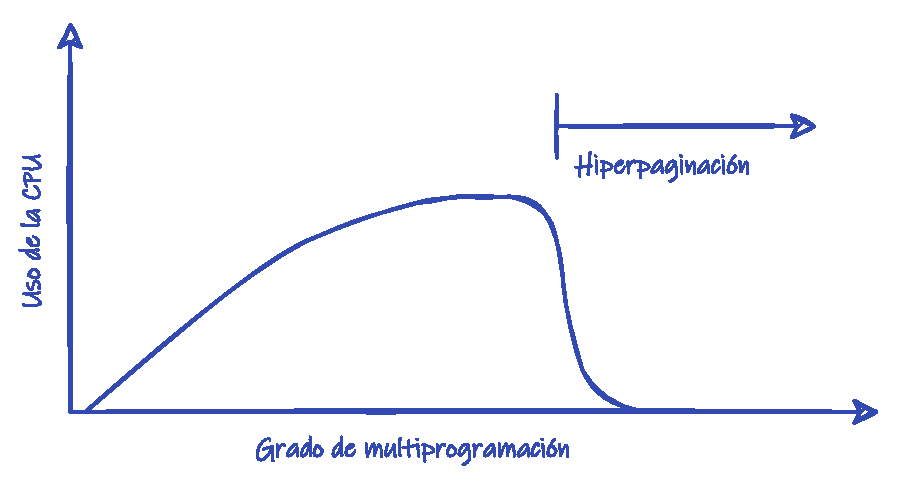
\includegraphics[width=0.8\textwidth]{media/C17_memoria_virtual/hiperpaginación.pdf}
\caption{Hiperpaginación en sistemas
multiprogramados.}\label{fig-hiperpaginaciuxf3n}
\end{figure}

El fenómeno comentado se ilustra en la
\hyperref[fig-hiperpaginaciuxf3n]{Hiperpaginación en sistemas
multiprogramados.}, donde se muestra el uso de la CPU frente al número
de procesos cargados en el sistema. Cuando esto último aumenta, el uso
de la CPU aumenta hasta alcanzar un máximo. Si el \textbf{grado de
multiprogramación} supera dicho punto, el sistema comienza a
\textbf{hiperpaginar}, por lo que el uso de la CPU disminuye
bruscamente.

Una solución es introducir un \textbf{planificador de medio plazo} que
detecte si el sistema está \textbf{hiperpaginando}, en cuyo caso
suspende y saca algunos procesos de la memoria ---reduciendo así el
\textbf{grado de multiprogramación}--- con el objeto de liberar memoria
para el resto de procesos en ejecución.

\subsection{Hiperpaginación en sistemas operativos
modernos}\label{_hiperpaginaciuxf3n_en_sistemas_operativos_modernos}

Los \textbf{sistemas de tiempo compartido} posteriores y los
\textbf{sistemas operativos modernos} no tienen ni \textbf{planificador
de largo plazo} ni \textbf{cola de entrada}, por lo que no ocurre el
efecto en cadena descrito en el caso de los sistemas multiprogramados.
Sin embargo, puede ocurrir la \textbf{hiperpaginación} si se ejecutan
demasiados procesos simultáneamente, de forma que alguno de ellos no
disponga de suficientes marcos para alojar todas las páginas que utiliza
frecuentemente (véase el
\hyperref[_modelo_del_conjunto_de_trabajo]{Modelo del conjunto de
trabajo}), aumentando así la \textbf{tasa de fallos de páginas}, hasta
el punto en que el proceso pasa más tiempo paginando que ejecutándose.

Los sistemas operativos modernos suelen carecer de \textbf{planificador
de medio plazo} por lo que, a diferencia de los \textbf{sistemas
multiprogramados}, no suspenden completamente la ejecución de algunos
procesos para reducir el consumo de memoria y evitar la
\textbf{hiperpaginación}. En su lugar, utilizan técnicas de memoria
virtual para ajustar la cantidad de marcos asignados a cada proceso,
intentando evitar la \textbf{hiperpaginación}, al tiempo que maximizan
el número de procesos que se pueden ejecutar simultaneamente.

En cualquier caso, como veremos en el
\hyperref[_modelo_del_conjunto_de_trabajo]{Modelo del conjunto de
trabajo}, habrá \textbf{hiperpaginación} si la cantidad mínima total de
marcos que necesitan todos los procesos para evitar la
\textbf{hiperpaginación} excede el número de marcos disponibles en el
sistema.

\subsection{Soluciones a la
hiperpaginación}\label{_soluciones_a_la_hiperpaginaciuxf3n}

Para el problema de la \textbf{hiperpaginación} existen diversas
soluciones:

\begin{itemize}
\item
  La principal solución es proporcionar a un proceso tantos marcos como
  le hagan falta. Como ya hemos comentado en diversas ocasiones, para
  evitar la \textbf{hiperpaginación} es necesario asignar al proceso al
  menos un número mínimo de marcos, que a priori no es conocido, ya que
  depende de cómo se comporta el proceso en su uso de la memoria. Una de
  las estrategias que pretenden estimar dicho número es el
  \textbf{modelo de conjunto de trabajo}, que veremos en la
  \hyperref[_modelo_del_conjunto_de_trabajo]{Modelo del conjunto de
  trabajo}.
\item
  Utilizar un algoritmo \textbf{de reemplazo local} puede limitiar el
  problema, pues de esta manera un proceso que \textbf{hiperpagina} no
  puede quitar marcos a otro, quizás incrementando su \textbf{tasa de
  fallos de página} y causando que también \textbf{hiperpagine}.

  Sin embargo, un algoritmo de \textbf{reemplazo local} no evita
  completamente que un proceso que \textbf{hiperpagine} afecte a otros.
  El uso intensivo del \textbf{dispositivo de intercambio}, por parte
  del proceso \textbf{hiperpagina}, puede afectar al rendimiento del
  sistema al aumentar el \textbf{tiempo de acceso efectivo} al disco.
\end{itemize}

\subsection{Modelo del conjunto de
trabajo}\label{_modelo_del_conjunto_de_trabajo}

{} Para entender el modelo de conjunto de trabajo es necesario comenzar
definiendo el \textbf{modelo de localidad}{}. El \textbf{modelo de
localidad} establece que:

\begin{itemize}
\item
  Una \textbf{{}localidad} es un conjunto de páginas que se utilizan
  juntas.
\item
  Cuando un proceso se ejecuta, se va moviendo de una \textbf{localidad}
  a otra.
\end{itemize}

Por ejemplo, cuando se invoca una función se define una nueva
\textbf{localidad}. En esta \textbf{localidad} las referencias a la
memoria se realizan: al código de la función, a las variables locales de
la misma y a algunas variables globales del programa.

Supongamos que proporcionamos a un proceso suficientes marcos como para
alojar toda su \textbf{localidad} en un momento dado. Entonces, el
proceso generará \textbf{fallos de página} hasta que todas las páginas
de su \textbf{localidad} estén cargadas. Después de eso no volverá a
fallar hasta que no cambie a una nueva \textbf{localidad}. Sin embargo,
si damos al proceso menos marcos de los que necesita su
\textbf{localidad}, este \textbf{hiperpaginará}.

El \textbf{modelo de conjunto de trabajo} es una estrategia que permite
obtener una aproximación de la \textbf{localidad} del programa y
consiste en lo siguiente:

\begin{itemize}
\item
  Definir el parámetro \emph{Δ} como el tamaño de la \textbf{ventana del
  conjunto de trabajo}.
\item
  En un instante dado, el conjunto de páginas presente en las \emph{Δ}
  últimas referencias a la memoria se consideran el \textbf{{}conjunto
  de trabajo}.
\item
  Por lo tanto, el \textbf{conjunto de trabajo} es una aproximación de
  \textbf{localidad} del programa.
\end{itemize}

Por ejemplo, dada la siguiente lista de referencias a páginas en la
memoria:

\begin{figure}
\centering
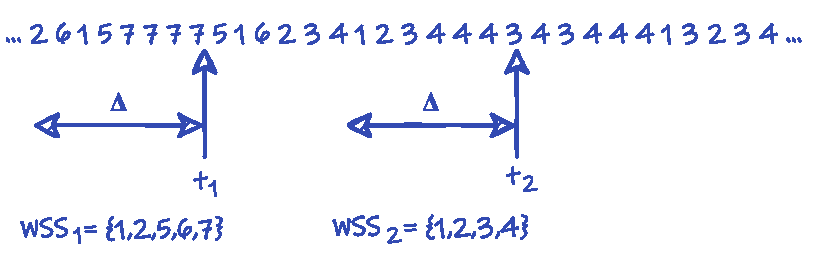
\includegraphics[width=0.8\textwidth]{media/C17_memoria_virtual/modelo_de_conjunto_de_trabajo.pdf}
\caption{}
\end{figure}

si \emph{Δ} = 10 referencias a la memoria, entonces el conjunto de
trabajo en \emph{t}\textsubscript{1} es \{1, 2, 5, 6, 7\}. Mientras que
en \emph{t}\textsubscript{2} el conjunto de trabajo es \{1, 2, 3, 4\}.

Obviamente, la precisión del \textbf{conjunto de trabajo} como
aproximación de la \textbf{localidad} del programa depende del parámetro
\emph{Δ}:

\begin{itemize}
\item
  Si \emph{Δ} es muy pequeña, el \textbf{conjunto de trabajo} no
  cubriría toda la \textbf{localidad}.
\item
  Si \emph{Δ} es muy grande, el \textbf{conjunto de trabajo} se
  superpondría a varias \textbf{localidades}.
\end{itemize}

\subsection{Uso del conjunto del trabajo para evitar la
hiperpaginación}\label{_uso_del_conjunto_del_trabajo_para_evitar_la_hiperpaginaciuxf3n}

El uso del conjunto de trabajo es bastante sencillo:

\begin{enumerate}
\def\labelenumi{\arabic{enumi}.}
\item
  Los diseñadores del sistema seleccionan \emph{Δ}.
\item
  El sistema operativo monitoriza el \textbf{conjunto de trabajo} de
  cada proceso y le asigna tantos marcos como páginas haya en el
  \textbf{conjunto de trabajo}.
\item
  Si sobran globalmente suficientes marcos:

  \begin{itemize}
  \item
    En el caso de los \textbf{sistemas multiprogramados}, otro proceso
    puede ser cargado desde la \textbf{cola de entrada} o desde el
    \textbf{dispositivo de intercambio}, si había sido suspendido
    previamente por el \textbf{planificador de medio plazo}.
  \item
    En sistemas más modernos la memoria libre puede destinarse a otros
    usos, como caché o búferes de E/S.
  \end{itemize}
\item
  Si el \textbf{tamaño del conjunto de trabajo} total \emph{WSS} crece y
  excede el número de marcos disponibles:

  \begin{itemize}
  \item
    En los \textbf{sistemas multiprogramados} con \textbf{planificador
    de medio plazo}, el sistema podría seleccionar un proceso para ser
    suspendido. Este volverá a ser cargado y reiniciado más tardel,
    cuando haya suficientes marcos libres.

    \begin{enumerate}
    \def\labelenumii{\alph{enumii}.}
    \item
      Los sistemas operativos más modernos reparten los marcos
      disponibles entre todos los procesos. Al ser la cantidad de marcos
      disponibles inferior al \emph{WSS}, es posible que algunos
      procesos \textbf{hiperpaginen}.
    \end{enumerate}
  \end{itemize}
\end{enumerate}

En la descripción anterior, el \textbf{tamaño del conjunto de trabajo}
\emph{WSS} es la suma del \textbf{tamaño de los conjuntos de trabajo}
\emph{WSS\textsubscript{i}} para cada proceso \emph{i}:

\[WSS=sum WSS_i\]

y representa la demanda total de marcos. Por eso, si \emph{WSS} es mayor
que el número de marcos disponibles, habrá \textbf{hiperpaginación}.

El sencillo algoritmo anterior permite evitar la
\textbf{hiperpaginación}. Sin embargo, el reto está en cómo mover la
\textbf{ventana del conjunto de trabajo} en cada referencia, con el fin
de volver a calcular el \textbf{conjunto de trabajo}.

Una posible aproximación es utilizar un temporizador que periódicamente
invoque a una función encargada de examinar el \textbf{bit de
referencia} de las páginas en la ventana de referencias \emph{Δ}. Es de
suponer que las páginas con el \textbf{bit de referencia} a 1 forman
parte de la \textbf{localidad} del programa y por tanto serán el
\textbf{conjunto de trabajo} a lo largo del siguiente periodo.

\section{Otras consideraciones}\label{_otras_consideraciones}

Ya hemos comentado que las principales decisiones que deben ser tomadas
en el diseño de un sistema con \textbf{paginación bajo demanda} son la
elección del \textbf{algoritmo de reemplazo} y la de la
\textbf{asignación de marcos de página}. Sin embargo, hay otras
consideraciones que deben ser tenidas en cuenta.

\subsection{Prepaginado}\label{_prepaginado}

El \textbf{{}prepaginado} es una técnica que consiste en cargar
múltiples páginas junto con la página demandada en cada \textbf{fallo de
página}.

Esas otras páginas se escogen especulativamente bajo la hipótesis de que
van a ser necesitadas por el proceso en un corto espacio de tiempo. De
manera que si la predicción es acertada, la \textbf{tasa de fallos de
página} se reduce significativamente. Esta técnica puede ser utiliza,
por ejemplo, en las siguientes situaciones:

\begin{itemize}
\item
  En la \textbf{paginación bajo demanda pura}, el sistema sabe de
  antemano que cuando se inicia un proceso siempre fallan las primeras
  páginas de código, por lo que son buenas candidatas para el
  \textbf{prepaginado}.
\item
  En el acceso secuencial a \textbf{archivos mapeados en memoria}.

  El sistema puede determinar que el acceso va a ser de tipo secuencial,
  tanto mediante el uso de técnicas heurísticas como mediante las
  opciones indicadas por el proceso en la llamada al sistema con la que
  se abrió el archivo.

  En cualquier caso, si el sistema determina que el acceso al archivo es
  secuencial, en cada \textbf{fallo de página} puede cargar tanto la
  página demanda como las siguientes, en previsión de que vayan a ser
  utilizadas por el proceso.
\end{itemize}

En general, el único inconveniente del \textbf{prepaginado} es que debe
ser ajustado para que el coste del mismo sea inferior al de servir los
\textbf{fallos de página}.

\subsection{Sobrereserva}\label{_sobrereserva}

{} {} Como las páginas de memoria de los procesos no necesitan memoria
física hasta que son referenciadas, los sistemas operativos con memoria
virtual pueden aceptar solicitudes de reserva de memoria aunque no haya
suficiente memoria física disponible. Para que el sistema operativo
pueda garantizar que siempre tiene dónde almacenar cualquier página de
cualquier proceso, debe asegurarse de que la cantidad total de memoria
reservada no exceda el espacio total disponible entre la memoria física
y el \textbf{espacio de intercambio}. Por lo general, si una petición de
reserva de memoria excede el espacio total disponible, el sistema
operativo la rechazará.

Si embargo, algunos sistemas operativos pueden aceptar solicitudes de
reserva de memoria que excedan el espacio total disponible. En estos
casos, el sistema operativo acepta la solicitud, pero no garantiza que
la memoria reservada pueda ser utilizada. Es lo que se conoce como
\textbf{sobrereserva} u \textbf{\textbf{overcommit}}.

Muchas distribuciones de Linux hacen \textbf{sobrereserva} por defecto,
aunque este comportamiento se puede desactivar. Desactivar la
\textbf{sobrereserva} es especialmente recomendable en sistemas
críticos, donde no se puede permitir que el sistema operativo termine
los procesos de forma prematura si el sistema se quedan sin espacio para
almacenar las páginas de memoria.

La \textbf{sobrereserva} es útil porque algunos programas reservan más
memoria de la que realmente necesitan, por lo que no tiene sentido que
se compruebe si hay suficiente espacio hasta que el proceso no utilice
realmente la memoria reservada. Sin embargo, tiene el riesgo de que si
se reserva más memoria de la disponible y todos los procesos intentan
utilizar buena parte de ella, el sistema se quede sin espacio para
almacenar las páginas de memoria y tenga que terminar procesos de forma
prematura para liberar espacio.

En los sistemas Linux, \textbf{{}Out Of Memory Killer} u \textbf{{}OOM
Killer} es el nombre que recibe la tarea del núcleo encargada de
terminar procesos cuando el sistema se queda sin memoria. El \textbf{OOM
Killer} selecciona los procesos a terminar en función de una serie de
criterios, como el uso de la CPU, la cantidad de memoria que consumen o
si el proceso es un servicio o un proceso de usuario.

\subsection{Aplicaciones en modo RAW}\label{_aplicaciones_en_modo_raw}

Algunas aplicaciones, cuando acceden sus datos a través de los
mecanismos de memoria virtual del sistema operativo, ofrecen peor
rendimiento del que conseguirían si este mecanismo no existiera.

El ejemplo típico, son los gestores de bases de datos, que conocen sus
necesidades de memoria y disco mejor que cualquier sistema operativo de
propósito general, por lo que salen beneficiadas si implementan sus
propios algoritmos de gestión de la memoria y de \emph{buffering} de
E/S.

Por eso muchos sistemas operativos modernos permiten que los programas
que lo soliciten puedan acceder a los discos en \textbf{modo RAW}. En el
\textbf{modo RAW} no hay sistema de archivos, ni paginación bajo
demanda, ni bloqueo de archivos, ni prepaginación, ni muchos otros
servicios del sistema operativo; por lo que dichas aplicaciones deben
implementar sus propios algoritmos de almacenamiento y gestión de la
memoria.

Sin embargo, hay que valorar muy bien las necesidades del programa antes
de optar por este modo. La mayor parte de las aplicaciones siempre
funcionan mejor utilizando los servicios convencionales ofrecidos por el
sistema operativo.

\subsection{Tamaño de las páginas}\label{_tamauxf1o_de_las_puxe1ginas}

Como ya comentamos al estudiar el método básico de paginación (véase el
\hyperref[paginaciuxf3n]{???}), una decisión de diseño importante es
escoger el tamaño adecuado para las páginas:

\begin{itemize}
\item
  \textbf{Con páginas grandes}:

  \begin{itemize}
  \item
    Se consiguen menos \textbf{fallos de páginas}. Por ejemplo, en un
    caso extremo, un proceso de 100 KiB solo podría generar un
    \textbf{fallo de página} si cada página es de 100 KiB, pero puede
    generar 102400 fallos si cada página es de 1 byte.
  \item
    Se consiguen tablas de páginas más pequeñas.
  \item
    La E/S para acceder al contenido de cada página requiere menos
    tiempo.

    En general el tiempo de transferencia es proporcional a la cantidad
    de información transferida, lo que debería beneficiar a los sistemas
    con páginas de pequeño tamaño. Sin embargo, la latencia y el tiempo
    requerido para posicionar la cabeza lectora de los discos es muy
    superior al tiempo de transferencias de datos, por lo que es más
    eficiente tener menos transferencias de mayor tamaño ---como cuando
    se usan páginas grandes--- que más transferencias de menor tamaño
    ---como cuando se usan páginas pequeñas---.
  \end{itemize}
\item
  \textbf{Con páginas pequeñas}:

  \begin{itemize}
  \item
    Se consigue tener menos \textbf{fragmentación interna} y, por tanto,
    un mejor aprovechamiento de la memoria.
  \item
    Teóricamente, se obtiene una mejor resolución para asignar y
    transferir al disco solo la memoria que realmente necesitamos. Esto
    a la larga debería redundar en menos memoria asignada y menos
    operaciones de E/S.
  \end{itemize}
\end{itemize}

En la actualidad, el tamaño de página más común es de 4 KiB en sistemas
de 32 bits y 8 KiB en los de 64 bits, ya que son adecuados para la mayor
parte de las aplicaciones. Sin embargo, muchos sistemas modernos
soportan el uso simultáneo de múltiples tamaños de página. Esto permite
que la mayor parte de las aplicaciones utilicen el tamaño estándar,
mientras las que hacen un uso intensivo de la memoria ---como es el caso
de los gestores de bases de datos--- puedan utilizar páginas de mayor
tamaño.

\subsection{Efecto de la estructura de los
programas}\label{_efecto_de_la_estructura_de_los_programas}

Los programas creados considerando la \textbf{localidad de referencia}
pueden mejorar su rendimiento en los sistemas con \textbf{paginación
bajo demanda}.

Vamos a ilustrarlo con el siguiente ejemplo de un programa que
inicializa a 0 un \emph{array} de 128 por 128 elementos.

\begin{Shaded}
\begin{Highlighting}[]
\DataTypeTok{char}\NormalTok{ data}\OperatorTok{[][]} \OperatorTok{=} \KeywordTok{new} \DataTypeTok{char}\OperatorTok{[}\DecValTok{128}\OperatorTok{][}\DecValTok{128}\OperatorTok{];}

\ControlFlowTok{for} \OperatorTok{(}\DataTypeTok{int}\NormalTok{ j }\OperatorTok{=} \DecValTok{0}\OperatorTok{;}\NormalTok{ j }\OperatorTok{\textless{}} \DecValTok{128}\OperatorTok{;} \OperatorTok{++}\NormalTok{j}\OperatorTok{)}
\OperatorTok{\{}
  \ControlFlowTok{for} \OperatorTok{(}\DataTypeTok{int}\NormalTok{ i }\OperatorTok{=} \DecValTok{0}\OperatorTok{;}\NormalTok{ i }\OperatorTok{\textless{}} \DecValTok{128}\OperatorTok{;} \OperatorTok{++}\NormalTok{i}\OperatorTok{)}
  \OperatorTok{\{}
\NormalTok{    data}\OperatorTok{[}\NormalTok{i}\OperatorTok{][}\NormalTok{j}\OperatorTok{]} \OperatorTok{=} \DecValTok{0}\OperatorTok{;}
  \OperatorTok{\}}
\OperatorTok{\}}
\end{Highlighting}
\end{Shaded}

Un \emph{array} como el indicado es almacenado en filas:

\begin{Shaded}
\begin{Highlighting}[]
\NormalTok{data}\OperatorTok{[}\DecValTok{0}\OperatorTok{][}\DecValTok{0}\OperatorTok{],}\NormalTok{ data}\OperatorTok{[}\DecValTok{0}\OperatorTok{][}\DecValTok{1}\OperatorTok{],} \OperatorTok{...,}\NormalTok{ data}\OperatorTok{[}\DecValTok{0}\OperatorTok{][}\DecValTok{127}\OperatorTok{]}
\NormalTok{data}\OperatorTok{[}\DecValTok{1}\OperatorTok{][}\DecValTok{0}\OperatorTok{],}\NormalTok{ data}\OperatorTok{[}\DecValTok{1}\OperatorTok{][}\DecValTok{1}\OperatorTok{],} \OperatorTok{...,}\NormalTok{ data}\OperatorTok{[}\DecValTok{127}\OperatorTok{][}\DecValTok{127}\OperatorTok{]}
\end{Highlighting}
\end{Shaded}

De manera que si suponemos que el tamaño de cada página es de 128 bytes,
en el mejor de los casos cada fila estará almacenada en una página. Por
lo tanto:

\begin{itemize}
\item
  Si el sistema le asigna 128 marcos o más, el proceso solo generará 128
  fallos de página.
\item
  Si el sistema operativo le asigna un solo marco, el proceso tendrá
  16 384 fallos, aproximadamente.
\end{itemize}

Sin embargo, el ejemplo sería diferente si el bucle interno del programa
recorriera las columnas del \emph{array} y no las filas:

Pues se podrían a 0 primero todos los bytes de una misma página antes de
empezar con la siguiente. Esto reduciría el número de \textbf{fallos de
página} a 128, aunque el sistema operativo solo asigne un marco al
proceso.

Por lo tanto se puede concluir que:

\begin{itemize}
\item
  La selección cuidadosa de las estructuras de datos y de programación
  pueden mejorar la \textbf{localidad}, reduciendo la \textbf{tasa de
  fallos de páginas} y el tamaño del \textbf{conjunto de trabajo}. Por
  ejemplo, las estructuras de datos tipo pila tienen buena
  \textbf{localidad}, puesto que el acceso siempre se realiza en lo alto
  de las mismas. Sin embargo, las tablas de dispersión, obviamente,
  están diseñadas para dispersar las referencias, lo que produce una
  mala \textbf{localidad}.
\item
  La elección del lenguaje de programación también puede tener efecto.
  En los lenguajes como C y C++ se utilizan punteros con frecuencia, lo
  que aleatoriza el acceso a la memoria, empeorando la \textbf{localidad
  de referencia}. Además, algunos estudios indican que los lenguajes
  orientados a objetos tienden a tener peor \textbf{localidad de
  referencia} que los que no lo son.
\item
  El compilador y el cargador también pueden tener un efecto importante:

  \begin{itemize}
  \item
    Separando el código de los datos para permitir que las páginas de
    código puedan ser de solo lectura. Esto es interesante porque las
    páginas no modificadas no tienen que ser escritas antes de ser
    reemplazadas.
  \item
    El compilador puede colocar las funciones que se llaman entre sí en
    la misma página.
  \item
    El cargador puede situar las funciones en la memoria de tal forma
    que en lo posible no crucen los bordes de las páginas.
  \end{itemize}
\end{itemize}

\subsection{Interbloqueo de E/S y bloqueo de
páginas}\label{_interbloqueo_de_es_y_bloqueo_de_puxe1ginas}

Supongamos que un proceso solicita una operación de E/S sobre el
contenido del marco de alguna de las páginas de su espacio de
direcciones y que, antes de que la operación sea realizada, la página es
reemplazada mientras el proceso está esperando. En ese caso, la
operación de E/S se podría acabar realizando sobre una página que
pertenece a un proceso diferente, ya que la operación de E/S se realiza
sobre el marco en la memoria física.

Para evitarlo existen diversas soluciones:

\begin{itemize}
\item
  Se puede utilizar la memoria del núcleo como búfer en las operaciones
  de E/S.

  En una escritura, esto obliga a la llamada al sistema a copiar los
  datos desde las páginas del proceso a la memoria del núcleo, antes de
  solicitar la operación de E/S. Mientras que en las operaciones de
  lectura sería justo al contrario.
\item
  Cada página puede tener un \textbf{bit de bloqueo} que se utiliza para
  indicar qué páginas no pueden ser seleccionadas para reemplazo.
\end{itemize}

Además los \textbf{bits de bloqueo}{} se pueden utilizar en otras muchas
situaciones:

\begin{itemize}
\item
  Bloquear las páginas del núcleo para evitar que sean reemplazadas.
\item
  Bloquear las páginas que acaban de ser cargadas.

  Esto evita que un \textbf{fallo de página} en un proceso de mayor
  prioridad pueda reclamar el marco antes de que el proceso para el que
  se cargó la página originalmente sea reiniciado, desperdiciando el
  trabajo de cargarla y provocando un nuevo \textbf{fallo de página}.

  Para implementarlo, se puede poner el \textbf{bit de bloqueo} a 1
  cuando la página se carga, volviéndolo después a poner a 0 cuando el
  proceso es planificado por primera vez, tras el \textbf{fallo de
  página} que provocó la carga de la página.
\item
  En los sistemas con \textbf{tiempo real flexible}, se suele permitir
  que las tareas de tiempo real informen de cuáles son las páginas más
  importantes, con el fin de que sean bloqueadas para evitar que puedan
  ser reemplazadas.

  Para evitar riesgos, el sistema suele considerar estas solicitudes
  como «consejos de bloqueo». De esta manera el sistema es libre de
  descartar dichos consejos si el conjunto de marcos libres llega a ser
  demasiado pequeño o si un proceso pide bloquear demasiadas páginas.
\end{itemize}

\subsection{Espacio de intercambio}\label{_espacio_de_intercambio}

La memoria virtual es una técnica que surgió para permitir ejecutar
programas que no caben en la memoria física, cuando esta era un recurso
muy limitado. Actualmente, con la cantidad de memoria física disponible
en los sistemas modernos, surge la duda de si sigue siendo necesario
disponer de espacio de intercambio.

Para responder a esa pregunta, hay que tener en cuenta que las páginas
de memoria pueden clasificarse en alguna de las siguientes categorías:

\begin{itemize}
\item
  \textbf{Páginas de código y datos del núcleo} que siempre están en
  memoria, por lo que se bloquean para evitar que sean reemplazadas.
\item
  \textbf{Páginas de para el caché de datos de E/S} con el objeto de
  acelerar futuros accesos a los mismos. Estas páginas puede ser
  reemplazadas y su contenido se puede descartar sin problemas.
\item
  \textbf{Código de programas}, que son páginas de solo lectura, por lo
  que su contenido es siempre el mismo que el del archivo del ejecutable
  que contiene al programa.
\item
  \textbf{Páginas que mapean archivos en la memoria}, cuyo contenido es
  el mismo que el de alguna región de un archivo en disco que les sirve
  de respaldo. Cuando estas páginas son de solo lectura, su contenido
  puede ser descartado sin problema. Mientras que si permiten acceso de
  escritura, las modificaciones son escritas por el sistema operativo en
  el archivo mapeado.
\item
  \textbf{Páginas anónimas}, son aquellas que no corresponden con ningún
  archivo en disco. Eso incluye la pila, el montón o la memoria
  reservada dinámicamente con \texttt{malloc()}, \texttt{new} o
  \texttt{mmap()}.

  Como el contenido de estas páginas no está respaldado en disco, si se
  reemplazan, el sistema operativo debe guardar su contenido en el
  espacio de intercambio.
\end{itemize}

Tener suficiente espacio de intercambio asegura la igualdad de trato
entre las páginas de memoria, independientemente del tipo de página que
sean. Porque si un sistema no dispone de espacio de intercambio, no
puede reemplazar \textbf{páginas anónimas}, sin importar si su contenido
es accedido con poca frecuencia, lo que puede llevar a reemplazar
páginas más importantes para el rendimiento del sistema.

Veamos las situaciones más típicas en cuanto la demanda de memoria y
como afecta al sistema tener o no espacio de intercambio:

\subsubsection{Baja demanda de memoria}\label{_baja_demanda_de_memoria}

\begin{itemize}
\item
  \textbf{Con espacio de intercambio}: El sistema puede optar
  intercambiar memoria anónima raramente utilizada, por ejemplo, para
  aumentar la cantidad de memoria caché y otras optimizaciones.
\item
  \textbf{Sin espacio de intercambio}: No se puede intercambiar la
  memoria anónima, ya que está bloqueada en la memoria. Aunque esto
  puede no presentar un problema de inmediato, en algunos casos puede
  implicar una caída en el rendimiento debido a que las páginas anónimas
  usadas con menor frecuencia no se puede utilizar para cosas más
  importantes.
\end{itemize}

\subsubsection{Demanda moderada de
memoria}\label{_demanda_moderada_de_memoria}

\begin{itemize}
\item
  \textbf{Con espacio de intercambio}: En este caso, todos los tipos de
  memoria tienen la misma posibilidad de ser reemplazadas. Esto
  significa que hay mayores posibilidades de reemplazar una página que
  no vaya a ser reclamada rápidamente de nuevo.
\item
  \textbf{Sin espacio de intercambio}: Como las páginas anónimas están
  bloqueadas en la memoria, el reemplazo tiene que ocurrir en otro tipo
  de memoria, aunque contenga peores candidatos para el reemplazo. Por
  tanto, el sistema tenderá a reducir las páginas utilizadas como caché
  de E/S, perjudicando el rendimiento del acceso al almacenamiento, y
  hay más posibilidades de reemplazar una página que se necesitará
  pronto, aumentando la probabilidad de acabar \textbf{hiperpaginando}.
\end{itemize}

\subsubsection{Alta demanda de memoria}\label{_alta_demanda_de_memoria}

\begin{itemize}
\item
  \textbf{Con espacio de intercambio}: El sistema es más resiliente a
  picos temporales de demanda de memoria, ya que tiene libertad para
  escoger las mejores páginas para intercambio. En casos de agotamiento
  severo de la memoria, tiende a prologarse el tiempo desde que comienza
  la \textbf{hiperpaginación} hasta que el sistema deja de ser usable.
\item
  \textbf{Sin espacio de intercambio}: El sistema cae en la
  \textbf{hiperpaginación} más rápidamente, ya que las páginas anónimas
  están bloqueadas en la memoria y no pueden ser reclamadas. En los
  sistemas Linux, el \textbf{OOM Killer} se activa más rápidamente para
  recuperar memoria por la vía de terminar procesos en ejecución.
\end{itemize}

\section{Interfaz de gestión de la
memoria}\label{_interfaz_de_gestiuxf3n_de_la_memoria}

Gracias a la abstracción de las técnicas de memoria virtual ---como la
paginación bajo demanda--- desde el punto de vista de los procesos, en
cualquier sistema moderno prácticamente solo hace falta una llamada al
sistema para gestionar su espacio de direcciones virtual.

En los sistemas POSIX esta llamada es \{linux\_mmap\} y en Windows API
es \{win32\_virtualalloc\}, que se usan junto a sus opuestas
\{linux\_munmap\} y \{win32\_virtualfree\}, respectivamente.

Ambas funciones permiten:

\begin{itemize}
\item
  Reservar una porción del espacio de direcciones virtual del proceso.

  La llamada solo hace la reserva de un rango de direcciones para que
  pueda ser utilizado por el proceso ---es decir, que las páginas en ese
  rango sean válidas--- siendo el componente de paginación bajo demanda,
  el responsable de asignar la memoria física que lo respalda, cuando el
  proceso acceda a esas direcciones.
\item
  Establecer permisos ---lectura, escritura y ejecución--- opciones de
  compartición entre procesos, bloqueo de páginas en la memoria física,
  páginas de gran tamaño y otras opciones, en la región de memoria
  virtual a reservar.
\end{itemize}

Además, en los sistemas POSIX, \{linux\_mmap\} se utiliza también para
mapear archivos en regiones del espacio de direcciones virtual. Mientras
que en Windows API para esa función se utilizan llamadas diferentes,
como hemos visto.

Ambas funciones ofrecen una buena cantidad de funcionalidades, pero
operan a muy bajo nivel. Por eso en ambas la página es la unidad mínima
en la gestión de la memoria. Es decir, las regiones reservadas del
espacio de direcciones virtual, siempre deben comenzar en un borde de
página y su tamaño debe ser múltiplo del tamaño de página.

El problema es cómo compatibilizar eso, con las necesidades reales de
los programas, que durante su ejecución necesitan reservar y liberar
constantemente memoria para pequeños elementos, como: \emph{arrays},
cadenas de texto, estructuras u objetos. Para esos casos, utilizar
directamente \{linux\_mmap\} o \{win32\_virtualalloc\} no es una
solución, puesto que la fragmentación interna conlleva un importante
derroche de recursos.

\subsection{Anatomía del espacio de direcciones virtual del
proceso}\label{_anatomuxeda_del_espacio_de_direcciones_virtual_del_proceso}

Los procesos pueden utilizar diversas ubicaciones dentro de su espacio
de direcciones virtual para almacenar los datos que necesitan para su
ejecución (véase la \hyperref[fig-proceso-en-memoria-completo]{Anatomía
de un proceso en memoria.}):

\begin{figure}
\centering
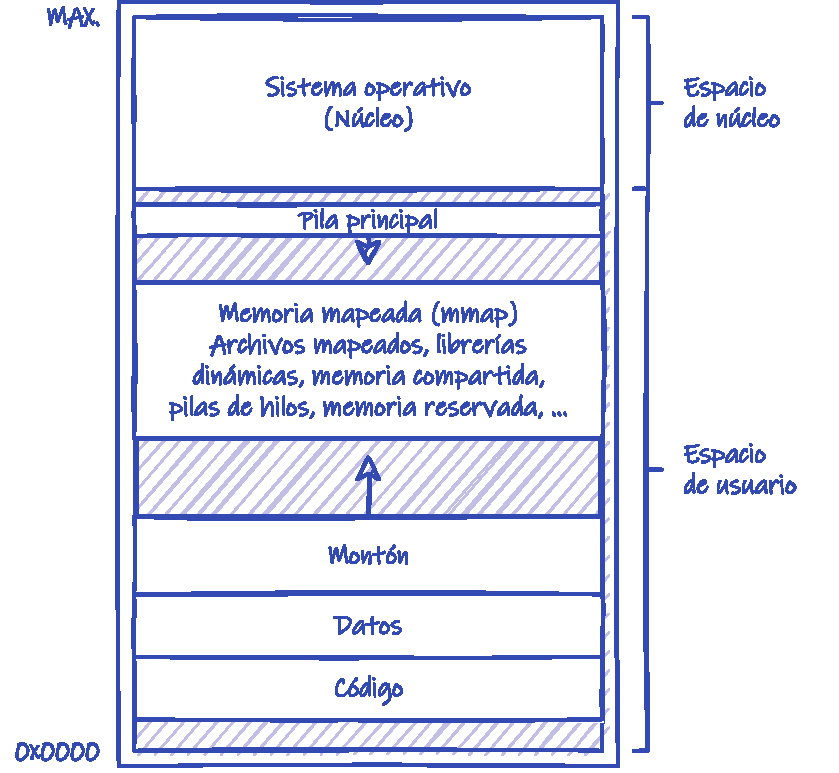
\includegraphics[width=0.8\textwidth]{media/C17_memoria_virtual/proceso_en_memoria_completo.pdf}
\caption{Anatomía de un proceso en
memoria.}\label{fig-proceso-en-memoria-completo}
\end{figure}

\begin{itemize}
\item
  Las variables y constantes globales se almacenan en el
  \textbf{segmento de datos}{}, que tiene tamaño fijo, ya que las
  dimensiones de estas variables se conocen de antemano en tiempo de
  compilación, al igual que ocurre con el código del programa.
\item
  Las variables locales y los argumentos de las funciones se almacenan
  en la \textbf{{}pila}, junto con las direcciones de retorno para
  volver de las funciones.

  Esta es la ubicación ideal para ellos, puesto que al retornar de una
  función, la pila se restablece al estado previo al que tenía cuando se
  invocó dicha función, haciendo que las variables locales y argumentos
  desaparezcan automáticamente.
\item
  Las variables reservadas dinámicamente ---por ejemplo, usando
  \{clang\_malloc\}/\{clang\_free\} en C o \{cpp\_new\}/\{cpp\_delete\}
  en C++ o Java--- se almacenan en el \textbf{{}montón}, que no es más
  una región contigua de memoria ubicada inmediatamente después del
  \textbf{segmento de datos} del proceso.
\item
  En la región entre el \textbf{montón} y la \textbf{pila} se ubican los
  \textbf{archivos mapeados en memoria}, las regiones de \textbf{memoria
  compartida}, las \textbf{librerías de enlace dinámico}, las
  \textbf{pilas} de cada hilo ---en procesos multihilo--- y, en general,
  la memoria reservada con funciones como \{linux\_mmap\} y
  \{win32\_virtualalloc\}.
\end{itemize}

Cada lenguaje de programación, debe proporcionar ---a través de su
\textbf{librería estándar}--- un mecanismo en espacio de usuario,
adecuado para la gestión en tiempo de ejecución de la memoria del
\textbf{montón} del proceso. Para eso, cada lenguaje puede utilizar su
propia implementación de dicho mecanismo o bien recurrir a la
proporcionada por la \textbf{librería del sistema}.

Por ejemplo, en los sistemas POSIX, la \textbf{librería del sistema}
proporciona su propia implementación, accesible a través de las
funciones \{clang\_malloc\} y \{clang\_free\}, que es utilizada
directamente por los programas escritos en C. Esta implementación hace
uso de \{linux\_mmap\}, pero ofrece mayor control sobre la cantidad de
memoria que podemos reservar, como veremos en el
\hyperref[_gestiuxf3n_de_la_memoria_del_montuxf3n]{Gestión de la memoria
del montón}.

Otros lenguajes de programación tienen otras interfaces para gestionar
la memoria, pero utilizan internamente las funciones \{clang\_malloc\} y
\{clang\_free\} de la \textbf{librería del sistema}. Sin embargo, este
no es el caso ni de C++ ni de Java ni de algunos otros lenguajes. En
C++, los operadores \{cpp\_new\} y \{cpp\_delete\} utilizan sus propios
algoritmos de gestión de la memoria del \textbf{montón}, más optimizados
que \{clang\_malloc\} y \{clang\_free\} para la creación y destrucción
de objetos de cualquier tamaño de manera eficiente.

En Windows API ocurre algo similar. La \textbf{librería del sistema}
proporciona su propia gestión de la memoria del \textbf{montón}, que es
accesible para cualquier programa a través de las funciones
\{win32\_heapalloc\} y \{win32\_heapfree\}, y que se implementa sobre
\{win32\_virtualalloc\}. La \textbf{librería estándar} de C utiliza, a
su vez, esas funciones para implementar \{clang\_malloc\} y
\{clang\_free\}. Lo mismo ocurre en otros lenguajes, aunque no en todos,
ya que algunos optan por implementar algoritmos más eficientes para sus
casos de uso directamente sobre \{win32\_virtualalloc\}.

\subsection{Gestión de la memoria del
montón}\label{_gestiuxf3n_de_la_memoria_del_montuxf3n}

Para ilustrar cómo se puede gestionar la memoria del \textbf{montón}
utilizaremos como ejemplo el mecanismo empleado por la \textbf{librería
del sistema} de los sistemas POSIX ---accesible a través de las
funciones \{clang\_malloc\} y \{clang\_free\}. Sin embargo, es
importante tener en cuenta que esta tarea se realiza de manera muy
similar en las implementaciones de otros sistemas operativos y lenguajes
de programación.

El funcionamiento básico de \{clang\_malloc\} sigue las siguientes
reglas:

\begin{enumerate}
\def\labelenumi{\arabic{enumi}.}
\item
  Cuando la memoria solicitada supera cierto umbral ---128 KiB en
  sistemas GNU/Linux--- es reservada directamente mediante la llamada al
  sistema \{linux\_mmap\}. Eso significa que las peticiones de gran
  tamaño realmente no consumen espacio del \textbf{montón}, si no que se
  reservan del hueco entre el \textbf{montón} y la \textbf{pila}.
\item
  Cuando un proceso hace una petición de memoria dinámica espera que el
  espacio ofrecido sea continuo en el espacio de direcciones virtual,
  por lo que la memoria del \textbf{montón} se gestiona usando un
  algoritmo de \textbf{asignación contigua de memoria} (véase
  \hyperref[_asignaciuxf3n_contigua_de_memoria]{???}) y, puesto que las
  peticiones pueden ser de tamaño variable, se utiliza con un esquema de
  \textbf{particionado dinámico}.

  Es decir, que para las peticiones que no entran en el caso anterior,
  se busca en la tabla de huecos libres y ocupados del \textbf{montón}
  uno lo suficientemente como grande para atender la petición. Se asigna
  el espacio solicitado y el resto sigue marcado como hueco libre.

  La estrategia más común de búsqueda es el \textbf{mejor ajuste},
  utilizando algún tipo de estructura de datos que mantenga los huecos
  libres ordenados por tamaño, para encontrar el de tamaño adecuado
  rápidamente.
\item
  Si no hay suficiente memoria libre contigua como para atender la
  petición, se utiliza la llamada al sistema \{linux\_mmap\}, para
  extender el tamaño del \textbf{montón} reservando una nueva región
  separada ---a veces llamada \textbf{{}arena}--- y comenzar a
  repartirla.
\end{enumerate}

En aplicaciones pequeñas, algunas implementaciones intentan ampliar
primero el espacio libre utilizando la llamada al sistema
\{linux\_brk\}, que sirve para extender el \textbf{montón} sobre la
región adyacente no asignada del espacio de direcciones virtual del
proceso. Este es el caso de la implementación estándar de
\{clang\_malloc\} en GNU/Linux.

La llamada al sistema \{linux\_brk\} ha sido eliminada del estándar
POSIX, pero algunos sistemas la mantienen por compatibilidad hacia
atrás, dado que era la forma en la que tradicionalmente se ampliaba la
memoria del \textbf{montón} en los primeros UNIX. En macOS esta llamada
se emula con una región de 4 MiB reservada con \textbf{mmap} la primera
vez que se utiliza.

La función \{clang\_calloc\} permite obtener memoria del \textbf{montón}
inicializada a 0, por lo que sigue las mismas reglas que
\{clang\_malloc\}. Cuando la petición es pequeña, obtiene la memoria del
\textbf{montón} ---extendiéndolo si fuera necesario--- para luego
ponerla manualmente a 0 antes de retornar de la función. Si la cantidad
es grande ---mayor de 128 KiB en sistemas GNU/Linux, como hemos
comentado--- obtiene la memoria llamando directamente a \{linux\_mmap\},
que ya la devuelve inicializada a 0 y que usa técnicas como el
\textbf{\emph{copy-on-write}} para ahorrar memoria física, retrasando la
asignación de marcos hasta el momento en el que el proceso comienza a
escribir realmente en la memoria reservada.

\subsection{Fragmentación}\label{_fragmentaciuxf3n}

La estrategia comentada sufre de \textbf{fragmentación interna}. En las
peticiones grandes, \{linux\_mmap\} reserva en múltiplos de tamaño de
página, por lo que siempre se puede perder cierta cantidad, aunque
pequeña en comparación al tamaño de la región reservada. En las
peticiones pequeñas, la memoria se asigna en múltiplos de una unidad
mínima ---por ejemplo, 16 o 32 bytes--- por lo que también se puede
perder cierta cantidad de memoria.

Además sufre de \textbf{fragmentación externa}, porque después de que el
proceso lleva un tiempo en ejecución, liberando y reservando memoria, el
espacio puede comenzar a quedar fraccionado en un gran número de
pequeños huecos, obligando a la librería a buscar más espacio para el
\textbf{montón}, aunque en suma haya suficiente espacio en los huecos
libres.

Esto representa un reto para los desarrolladores de aplicaciones, que
previsiblemente vayan a ejecutarse durante periodos muy largos de
tiempo. En esos casos, es común optar por librerías externas, que
implementen gestores de memoria que fragmenten menos la memoria, o
soluciones basadas en alguna forma de referencias indirectas y
recolección de basura, para ocasionalmente poder compactar la memoria
del \textbf{montón}. Esto último, es lo que hace la máquina virtual de
Java.
